\hypersetup{pdfborder=0 0 0}
%\vspace{10\baselineskip}

%\selectlanguage{french}
%----------------------------------------------------------------------
\section{Résumé (en français)}
%----------------------------------------------------------------------

Ce chapitre concerne l'étude de la dynamique de fine échelle du détroit de Gibraltar, d'une part par l'intermédiaire des résultats d'une maquette numérique dites haute résolution (section \ref{sectionSim3D}), d'autre part par l'analyse de quelques observations \textit{in situ} effectuées au cours de la campagne de mesure Gibraltar 2020 (section \ref{sectionCampagne}).

Les simulations analysées dans la section \ref{sectionSim3D} sont dans la continuité de celles présentées dans le chapitre \ref{chapGBR2D}. Aucun forçage atmosphérique n'est intégré ici, cependant le flot est tri-dimensionnel et prend en compte des forçages réalistes par le biais d'une initialisation et des forçages aux frontières issues du modèle opérationnel de l'ENEA, et d'une bathymétrie haute résolution. La stratification des masses d'eaux et les ondes de marées sont réalistes.

En particulier, il est possible de reconstituer un cycle mortes-eaux / vives-eaux. Trois périodes de simulations sont analysées correspondant à une morte-eau (SimNT), une vive-eau (SimST), et la partie croissante du cycle (SimIT).

L'analyse s'effectue par le biais de divers diagnostiques mis au point au cours de la thèse. Elle est ici focalisée sur la variabilité par rapport à l'intensité du forçage de la marée semi-dirune. Les différentes configurations de l'écoulement des masses d'eaux méditerranéennes et atlantiques concerannt leur statut sub/supercritique sont présentées. 

Plusieurs résultats sont mis en évidence dans ces simulations. Tout d'abord, 3 configurations du flot au Seuil de Camarinal sont repérées pour les périodes dites d'\textit{outflow}, selon la présence ou non, et la position du ressaut hydraulique établi lors des transitions entre flot supercritique et subcritique des eaux Atlantique. Ces configurations sont no-jump (pas de ressaut détecté), s-jump (ressaut à l'aplomb de la partie la moins profonde du Seuil) et w-jump (ressaut placé au-dessus de la pente ouest du seuil).

Les marées à plus faible amplitude de mortes-eaux correspondent à une situaion no-jump, les plus fortes de vives-eaux à la situation w-jump. La situation s-jump est un cas intermédiaire. On repère sur les simulations que la relaxation du ressaut hydraulique r"sulte bien en la propagation d'un train d'onde solitaires. Cependant, il est aussi vu que la propagation de l'onde longue de marée barocline à travers le détroit sans présence préalable de ressaut (cas no-jump) peut aboutir à un comportement non-linéaire qui dégénère en un soliton. Dans ce cas, le nombre de solitons du train se propageant en Mer d'Alboran est réduit, l'amplitude de l'anomalie de profondeur de l'interafce initiale étant réduite.

Outre la propagation du soliton, la haute résolution est tout comme c'était le cas au chapitre \ref{chapGBR2D} de simuler des instabilités de cisaillement dans le courant de densité à l'ouest du Seuil de Camarinal durant les périodes d'outflow. Leurs zones probables de génération ne changent pas entre les cas no-jump et s-jump et sont centrées sur les deux sillons nord et sud de parte t d'autre du point culminant du seuil de camarinal. Dans le cas w-jump, cette genération se fait à toutes les latitudes.

La comparaison de la simulation de ces instabilités par divers schémas de fermeture turbulente (Smagorinsky avec ajustement du coefficent, GLS) met en exergue leur rôle dans la composition hydraulogique de l'outflow méditerranéen en pilotant l'injection de'aux atlantiques.

LA dynamique de ces simulations a aidé à préparer la Campagne Gibraltar 2020, qui a eu lieu en Octobre 2020.

Les observations présentées dans la section \ref{sectionCampagne} sont essentiellement des données issues de trois mouillages, un au seuil de Camarinal, deux juste à l'est qui interceptent le soliton se propageant après relaxation du ressaut hydrauliques. Ces mouillages sont posés ... ... . Ici, seule la première période est présentée. Cinq types de signaux sont repérés. Trois d'entre eux ne sont pas liés à la propagation de solitons.

ce resultat semble conforme auw simulations, ou sur des outflow sans ressaut, pouvaitbtout de meme avoir des ... ce qui indiquerait que le ressaut n’est pas le seul mecanisme de generation pourbles solitons observes en mervd’alboran.




%----------------------------------------------------------------------
\section{3D LES in the Strait of Gibraltar}
%----------------------------------------------------------------------
\label{sectionSim3D}
\subsection{Introduction}

The Atlantic - Mediterranean exchange occurring in the Strait of Gibraltar has been explored summarily in a previous section (section \ref{sectionSim2D}). The consequences at basin scale broadly consists in Mediterranean waters leaving the Strait at depth (as what has been dubbed the 'Mediterranean outflow') whereas Atlantic waters enter the Mediterranean basin in the surface layer.

Those Atlantic waters entering through the Gibraltar Strait are the principal contribution to the Mediterranean inflowing water budget: the average transport of Atlantic waters at Gibraltar is of the order of 1 Sv whereas the net exchange itself is of the order of 0.1 Sv. This positive entry offsets the otherwise net evaporation occurring on the integrated surface over the Mediterranean basin \citep{bryden_1994}.
Since the Mediterranean basin is otherwise a closed, Mediterranean waters leaving the Strait of Gibraltar are the result of the transformations of the surface circulating Atlantic water mass into intermediate and deep water masses in the various seas.
More details are provided in this section on the characteristics of the strait, on the exchange, its variability, and on the fine-scale processes that take place during this exchange.\\
A clear objective of the numerical approach proposed in the present chapter is the explicit representation of these fine scales in the Strait of Gibraltar in order to better simulate the route toward mixing in this peculiar region of the ocean. Large Eddy Simulation (LES) is implemented to simulate the primary instabilities developing at depth between the Mediterranean and Atlantic water masses.

%----------------------------------------------------------------------
\subsubsection{Circulation in neighbouring areas (Gulf of Cadix and Alboran Sea)}
%----------------------------------------------------------------------

\subparagraph{Atlantic side of the Strait of Gibraltar.}

The surface waters that enter the strait are North Atlantic Central Water (NACW) and South-Atlantic Waters (SAW) \citep{millot_2014,naranjo_2015}. They are carried by the Portugal and Azores Currents into the Strait of Gibraltar as part of the eastern branch of the north-Atlantic subtropical gyre \citep{barton_2001}.

The Mediterranean water mass that was transported out of the strait as the Mediterranean outflow circulates at depth below this surface circulation in the Northern Atlantic. This outflow first enters the Gulf of Cadix, turning north due to geostrophy and flowing along the continental slope \citep{price_1993,gasser_2017}. West of the Gulf of Cadiz, it stabilizes to its neutral buoyancy level at 1000-m depth as the "Mediterranean water mass"\citep{price_1993}.

Meddies are salty lenses of water with negative  \color{blue}(?) \color{black} vorticity that can persist for years and can be found far in the open ocean. \color{blue}They \color{black} are generated along the canyons and caps encountered by the Mediterranean outflow in the region of the Gulf of Cadiz \citep{bashmachnikov_2015}. 

The Mediterranean water mass participates in the global circulation in the Northern Atlantic overturning circulation. It increases the salinity of the whole Northern Atlantic basin by spreading in the open ocean, whether as slowly decaying meddies or as water carried by subsurface currents to join the basin scale circulation at higher latitudes \citep{price_1993,jia_2007}.

\subparagraph{Mediterranean side of the strait of Gibraltar.} 

Surface waters leaving the strait at the eastern end enter the Alboran Sea as the Atlantic Jet (AJ). The circulation of the Alboran sea can vary in time. The most common state is organized around two anticyclonic gyres: the Western Alboran Gyre (WAG) and the Eastern Alboran Gyre (EAG). However, it is not uncommon that only one of these two gyres is present \citep{millot_2005}. The WAG is coupled to the Atlantic jet and usually constitutes its northern branch.\color{red}In this case, upwelling(?)\color{black} The AJ variability is mainly due to meteorological and tidal forcing, and can destabilize this system \citep{sanchez-garrido_2013,lorente_2019}.

At depth, several components of the Mediterranean water masses enter the strait. In the Alboran Sea, they are identified as LIW (for Leventine Intermediate Water) and WMDW (for West Mediterranean Deep Water).  Additional water masses from the western Mediterranean basin like TDW (for Thryenian Deep Water) have also been detected \citep{millot_2014}. A zonal(\color{blue}meridional???\color{black}) organization of these water masses has been observed: TDW, LIW and other intermediate waters are \color{black} more abundant in the northern part of the Alboran sea, whereas WMDW is mostly present in its southern part \citep{millot_2014}. As the depth decreases from the Alboran sea to the Strait of Gibraltar, it is more difficult for deeper WMDW to pass through the strait, and its input can be regulated by mechanisms such as the strength of the WAG or the overall production of WMDW linked to the strength of winter convection \citep{naranjo_2012}.

\subparagraph{Transformation of the water masses.}
Both the inflowing (in reference to the Mediterranean basin) Atlantic waters or the outflowing (ditto) Mediterranean waters incorporate signatures of respectively the Mediterranean \citep{macias_2006} and Atlantic waters \citep{millot_2007,garcia-lafuente_2011}. This is due to the mixing driven by small-scale processes of variable strength occuring in the Strait of Gibraltar.  


%%%%%%%%%%%%%%%%%%%%%%%%%%%%%%%%%%%%%%%%%%%%%%%%%%%%%%%%%%%%%%%%%%%%%%%%%%%%
\subsubsection{Morphology, barotropic tides and atmospheric forcing.} 
%%%%%%%%%%%%%%%%%%%%%%%%%%%%%%%%%%%%%%%%%%%%%%%%%%%%%%%%%%%%%%%%%%%%%%%%%%%%%


The Strait of Gibraltar is tilted at approximately 15$^\text{o}$ compared to the east direction. Away from the continental shelf, Camarinal Sill (CS) is the shallowest point of the strait with an average depth of about 300 m (see figure \ref{FigBathy3D}). The strait is narrow and deep east of CS. The shallower west side of CS is divided by two troughs on each side of a submarine mount called Majuan Bank. The northern trough is shallower than the southern one, which includes another sill, called Espartel Sill (ES). Those two troughs are the main pathways the Mediterranean outflow takes to reach the Gulf of Cadix. Most of the flow takes the southern, deeper path \citep{soto-navarro_2015}.

The barotropic (M2) semi-diurnal tide flows from the North Atlantic basin and constitutes the foremost varying signal for the currents in the strait, propagating from south to north with an amplitude decreasing from west to east \citep{candela_1990}. During the flood (ebb) tide, barotropic currents are oriented westward (eastward). The currents associated with the barotropic tide have the same amplitude as the mean circulation. They can reverse the flow of Mediterranean and/or Atlantic waters in certain sections \citep{sanchez-roman_2012}, and they have a pronounced neap-spring tide cycle.

The wind is funneled through the strait and is principally zonal, either blowing westward or eastward with a speed reaching $25\ m/s$ \citep{candela_1989}. Wind stress affects only the first tens of meters of the circulation in the strait \citep{candela_1989}, which can be sufficient to affect the Atlantic jet, by inducing either an acceleration or a deceleration (sometimes even stopping the jet) \citep{lorente_2019}. The strength of the AJ then changes its tilt as it enters the Alboran Sea and how it interacts with the WAG. Otherwise, the integrated effect of atmospheric pressure over the Mediterranean basin can influence the net flow through the strait \citep{garcialafuente_2002}.



%%%%%%%%%%%%%%%%%%%%%%%%%%%%%%%%
\subsubsection{Baroclinic exchange and small-scale processes}


The circulation of eastward Atlantic waters at the surface and of westward Mediterranean waters at depth sets up a baroclinic exchange in the strait of Gibraltar. Due to the amplitude of the barotropic (tidal) currents, this exchange is intermittent with regard to the semi-dirunal tide. The circulation can thus be splitted into a low frequency time-average component of the mean exchange and a high-frequency, eddy-flux-like, tidal anomaly. The latter has an important impact on the exchange flow \citep{naranjo_2014}, and can even have a larger amplitude than the former at CS \citep{vargas_2006}.

The amplitude of the exchange varies over timescales larger than the semi-diurnal tide. The lower frequencies (whether seasonal or inter-annual) are usually linked to atmospheric forcing over the Mediterranean \citep{sanchez-roman_2012}. The tidal eddy-fluxes have their own variability associated to the spring-tide cycle and to the monthly tides, with for example a greater depth and stronger shear during neap tides, but more intense mixing during spring tide \citep{naranjo_2014,vargas_2006}.\color{red}(enlever? sert à rien? que dans intro plus générale???)\color{black}

Various small-scale processes can additionally be identified in the Strait of Gibraltar.\color{red}Sert pas..si enleveparagraphe d'avant.\color{black}

\color{red}Dire supercriticalité dû a ce fait que courant marée peuvent être aussi grand...

The flow at CS is .... cascading , new injection as density front. Additionally, the high celerity of the flow due to barotropic tide channeled means can have hydraulic control... also occurs elsewhere in the strait\color{black}

Firstly, due to the limited horizontal and vertical extent of the strait, the time-averaged exchange flow and the depth-averaged barotropic tidal currents are channeled in the strait. A consequence is that the flow in the strait can become supercritical in regard to internal gravity wave propagation meaning that the velocity of the currents are larger than the velocity of the internal gravity waves.  East (west) of CS, the flow in the Atlantic (resp. Mediterranean) layer becomes supercritical.



Hydraulic control of the exchange flow only occurs episodically at CS. More generally, the location and the variability of the occurrence of supercritical flows can yet vary depending on the type of diagnostics used to characterize such events (see for instance \citet{armi_1988,vargas_2006,sannino_2007,sanchez-roman_2012}). 

In the region of CS, the development of two hydraulic jumps when hydraulic control occurs reflects the geometry of the sill and can be observed on satellite imagery \citep{brandt_1996}. The hydraulic jump remains approximately 4 hours in the region of Camarinal during outflows \citep{armi_1988,vlasenko_2009}. During this particular period, an intense mixing of Mediterranean and Atlantic waters occurs \citep{wesson_1994,macias_2006,garcia-lafuente_2011}. Strong billows are indeed induced by Kelvin-Helmoltz instabilities in the lee of the hydraulic jump. These billows are then advected westward by the Mediterranean flow \citep{wesson_1994}. In addition, the establishment of the hydraulic jump matches with the presence of chlorophyll-rich waters in the center of the strait \citep{bruno_2013}.

When the tidal flow reverses toward the Mediterranean basin, the depressed anomaly of the interface between Mediterranean and Atlantic waters propagates as a Large Amplitude Internal Wave (LAIW). It takes the form of a solitary bore before transforming into an Internal Solitary Wave (ISW) \citep{armi_1988}. An ISW is a particular type of internal wave satisfying a balance between non-linear advection of momentum and non-hydrostatic dispersion, which makes the initial wave expand into a train of ISWs \citep{vlasenko_2000}. The signature of such solitary waves have been extensively observed both at the surface (as areas of alterning surface roughness) and at depth (as anomaly in tracer and velocity fields) (\citet{ziegenbein_1970,armi_1988,watson_1990,sanchezgarrido_2008} to cite a few). They transport chlorophyll \citep{bruno_2013} and they are expected to induce remote mixing in the Alboran sea.

ISWs are generated during each tidal cycle except when westward current are not strong enough for the hydraulic control to set up. This is for instance the case during the neap tide part of the forthnightly cycle\citep{watson_1990,garcialafuente_2000}. \color{red}Reformuler, c'ets naze................\color{black}

The hydraulic control, the hydraulic jump and the generation mechanism of large internal tides can be simulated numerically by hydrostatic models but a non-hydrostatic model is required to simulate the propagation of ISWs or the large turbulent eddies and primary instabilities induced by the baroclinic exchange flow \citep{brandt_1996,vlasenko_2009}.



%%%%%%%%%%%%%%%%%%%%%%%%%%%%%%%%%%%%%%%%%%%%%%
\subsubsection{Toward Large Eddy Simulation (LES)}

The small-scale processes are consequently responsible for the mixing of Atlantic and Mediterranean waters in the Strait of Gibraltar, and the characteristics of the water masses involved in the baroclinic exchange at Gibraltar are not conserved. It remains yet difficult to clearly isolate the retroaction of such small-scale processes on the circulation and more generally on the large-scale processes observed in the Mediterranean basin \citep{garcia-lafuente2017}.
The enhanced mixing in the strait must in any event be parameterized in coarsely-resolved global or even in regional models and the modification of water-mass characteristics has an impact on the circulation in both the Mediterranean and the northern Atlantic basins. 


\color{red}A similar high resolution .. is presented in ...(mettre dans conclusion)\color{black}

Based on the preliminary numerical study presented by \citet{hilt_2020} (chapter \ref{chapGBR2D} of the present manuscript), the 3D s-coordinate, non-hydrostatic, free-surface model CROCO is implemented in the region of Gibraltar with a horizontal resolution of a few tenths of meters. We should show that such a high resolution grid is sufficient to resolve at least the largest scales of the mixing processes in the strait, i.e. the largest turbulent eddies or primary instabilities. A specific focus is made on different tidal forcing configurations during a neap-spring tidal cycle and on the way the flow characteristics and the intensity of mixing processes are affected by this variability. 

The numerical simulation framework based on three simulation periods is presented in section \ref{section3Dnum}. Various diagnosis that have been implemented in the numerical experiments are described in section \ref{PartDiag3D}. Section \ref{section3DRes} presents results pertaining to : the hydrological state of the flow depending on the strength of barotropic tidal currents; the propagation of ISWs; the areas of generation of primary instabilities; and a comparison of several turbulence closure schemes.

%----------------------------------------------------------------------
\subsection{Numerical Configuration}
%----------------------------------------------------------------------
\label{section3Dnum}

\subsubsection{Numerical framework}

Numerical configurations are based on CROCO-NBQ and build on \citet{hilt_2020}, see section \ref{sectionSim2D}. Most numerical parameters are summarized in table \ref{tab_NH-HR}. A non-linear equation of state and a no-slip condition at the bottom have also been implemented. \color{blue} A simple Smagorinsky-like turbulent closure scheme ('Smago' in table \ref{tab_sim3Dnames}) with a characteristic Smagorinsky coefficient chosen equal to 0.05 (reference?) is used in most simulations as presented in \ref{tab_sim3Dnames}. In section (\S \ref{sectionsim3D_res_insta}), several other Smagorinsky coefficients are further tested  ($10{-3}$,$10{-2}$,$10^{-1}$), together with the use of a GLS k-$\epsilon$ turbulent closure scheme, to evaluate the consequences on the simulated dynamics.

A crucial aspect in the \color{red}elaboration/build\color{black} of such high-resolution numerical configurations of the Strait of Gibraltar is the realism (and quality) of \color{red}bathymetry\color{black} data. Indeed the topography of the strait has significant (not to say major) consequences on the local and regional dynamics. Here, a 100-m-resolved MNT SHOM bathymetry has been used and adapted to model requirements and is presented in figure \ref{FigBathy3D}.

Initialization and open-boundary conditions (which include tidal forcing) are based on a simulation of the operational Mediterranean and Black sea model by ENEA using MitGCM (ENEA, Rome)\footnote{http://www.enea.it/it/seguici/pubblicazioni/pdf-volumi/cresco-report-2016.pdf}. This ENEA configuration can be viewed as a parent simulation. It has a horizontal resolution in the strait of approximately 700 m with vertical z-levels (repartition? Ref). By contrast, the simulations discussed in the next sections have a horizontal resolution of 45 m and 40 evenly spaced vertical $\sigma$-levels. As noted in table \ref{tab_NH-HR}, this is sufficient to provide a higher resolution in the vertical direction than in the horizontal for the whole simulation domain. For exemple, at CS, vertical resolution varies from approximately 7.5 m at the shallowest point of the sill, to approximately 12.5 m downslope.\\

No wind forcing and no atmospheric fluxes are specified at the surface of the ocean in the studied configurations. This choice is not a consequence of any numerical constraints or malfunctions but is dictated by the will to address the complex dynamics of the region step-by-step, concentrating first on the exchange and tidal flow crossing Gibraltar strait and on the fine scales developing at depth in a realistic context (apart from the atmospheric forcing).\color{red}(changer de place, mettre dans section campagne, préparation) Complete, realistic configurations (including the atmospheric forcing) are eventually carried out to prepare Gibraltar campaigns, to deliver forecasts during the campaigns and hindcasts in order to further explore the processes observed during the 2020 Gibraltar campaign (see \S XXX).\color{black}

To somehow reduce the computing cost of the various numerical configurations, the first 6 hours can be considered as a spin-up period and are simulated with CROCO's hydrostatic kernel over the same 45-m-horizontal-resolution grid. The last field is used as a restart file to initialize the fully non-hydrostatic and compressible simulation. This 6-h spin-up is made necessary by the large ratio existing between the forcing grid length-scale of the MitGCM ENEA coarse-grid field and the CROCO grid length-scale (a ratio reaching 15 to 30 depending on the studied configurations). In the future, such a downscalling procedure should be implemented through a cascade of simulations. On top of the exploration of the fine-scale dynamics and of its retroaction on the larger-scale circulation, the present study is indeed framed in the numerical development of two-way downscalling of the region of the Strait of Gibraltar in basin-scale circulations models.

\begin{table}[!h]
        \centering
        \begin{tabular}{|p{\linewidth/3}|c|c|}
                \hline
                Grid Extension & \multicolumn{2}{c|} {6°4.8'W  5°3.4'W ;}\\
                & \multicolumn{2}{c|} {35°23.8'N  36°27.4'N}\\
                Number of horizontal grid points & \multicolumn{2}{c|} {2049x2621}  \\
                Number of vertical $\sigma$-levels & \multicolumn{2}{c|} {40} \\
                $\Delta x = \Delta y$ & \multicolumn{2}{c|} {45 m}\\
                Depth & Min & Max\\
                & 26 m & 960 m\\
                $\Delta$z & 0.7 m & 24 m\\
                Internal time-step ($\Delta t_s$) & \multicolumn{2}{c|} {1 s}\\
                External time-step ($\Delta t_f$) & \multicolumn{2}{c|} {1/11 s (change 1/14)}\\
                Advection scheme & \multicolumn{2}{c|} {WENO-5} \\
                Viscosity $\nu$ & \multicolumn{2}{c|} {10$^{-6}$ m$^2$/s} \\
                Diffusivity $K_\rho$(aussi Ks et Kt) & \multicolumn{2}{c|} {10$^{-6}$ m$^2$/s}\\
                Sound wave velocity $C_s$ & \multicolumn{2}{c|} {400 m/s}\\
                Tidal harmonics (from ENEA) & \multicolumn{2}{c|} { $\text{M}_{\text{2}}$, $\text{S}_{\text{2}}$,$\text{K}_{\text{1}}$, $\text{O}_{\text{1}}$ }\\
                \hline
        \end{tabular}
        \captionof{table}{Simulation parameters}
        \label{tab_NH-HR}
\end{table}

\begin{table}[!h]
        \centering
        \begin{tabular}{|c|c|}
                \hline
                Closure scheme & Simulation name\\
                \hline
                Smago 0.005 & SimIT, SimNT, SimST\\
                Smago 0.001 & SimIT-S001\\
                Smago 0.01 & SimIT-S01\\
                Smago 0.1 & SimIT-S1\\
                GLS K-$\epsilon$ & SimIT-Kep\\
                \hline
        \end{tabular}
        \captionof{table}{Simulation names and turbulent closure schemes}
        \label{tab_sim3Dnames}
\end{table}

\subsubsection{Tidal forcing and simulation period}
Tidal forcing is integrated to the forcing at the lateral eastern and western boundaries (the only open boundaries). As indicated in table \ref{tab_NH-HR}, it comprises four tidal harmonic components ($\text{M}_{\text{2}}$, $\text{S}_{\text{2}}$, $\text{K}_{\text{1}}$, $\text{O}_{\text{1}}$). To limit computational costs, simulations are run for two-day periods of 3 characteristic flow configurations of September, 2017 (i.e. close to equinox). The start and end dates of each CROCO simulation are prescribed in table \ref{tab_dates_MIV}. They do not include the 6-hour-hydrostatic spin-up period.

The comparison of the sea-level anomaly near Tarifa (5.6° West, 36.01° North) in both the parent MitGCM and CROCO simulations and the corresponding tidal gauge data (from Puertos del Estado\color{red}Ref!!!\color{black}) are shown in figure \ref{fig_maree_tar}. \color{blue} This comparison shows that the CROCO configurations remain close to parent MitGCM implementation except during the neap tide period. \color{red}Since in nep tide the relative importance of the tidal brotropic currents is reduced compared to the exchange, this may be due to differing symanics in the Strait itself (serait bien faire comparaison point hors du détroit...) \color{black}

\begin{table}[h]
        %\begin{minipage}{.6\textwidth}
        \centering
        \begin{tabular}{|c|c|c|}
                \hline
                Situation & Simulation name & Dates (UTC)\\
                \hline
                Intermediate Tide & SimIT & 10/09/2017 19h00 - 13/09/17 01h00  \\
                Neap Tide & SimNT & 13/09/2017 16h00 - 15/09/17 17h00 \\
                %\hline
                Spring Tide & SimST & 19/09/2017 22h00 - 21/09/17 23h00  \\
                \hline
        \end{tabular}
        \captionof{table}{\sout{Périodes de simulation pour les 3 sitituations VE, MM et ME} \color{blue}Start and end dates of CROCO HR simulations corresponding to intermediate, neap and spring tides..}
        \label{tab_dates_MIV}
        %\end{minipage}
\end{table}

\begin{figure}[!h]
        \centering
        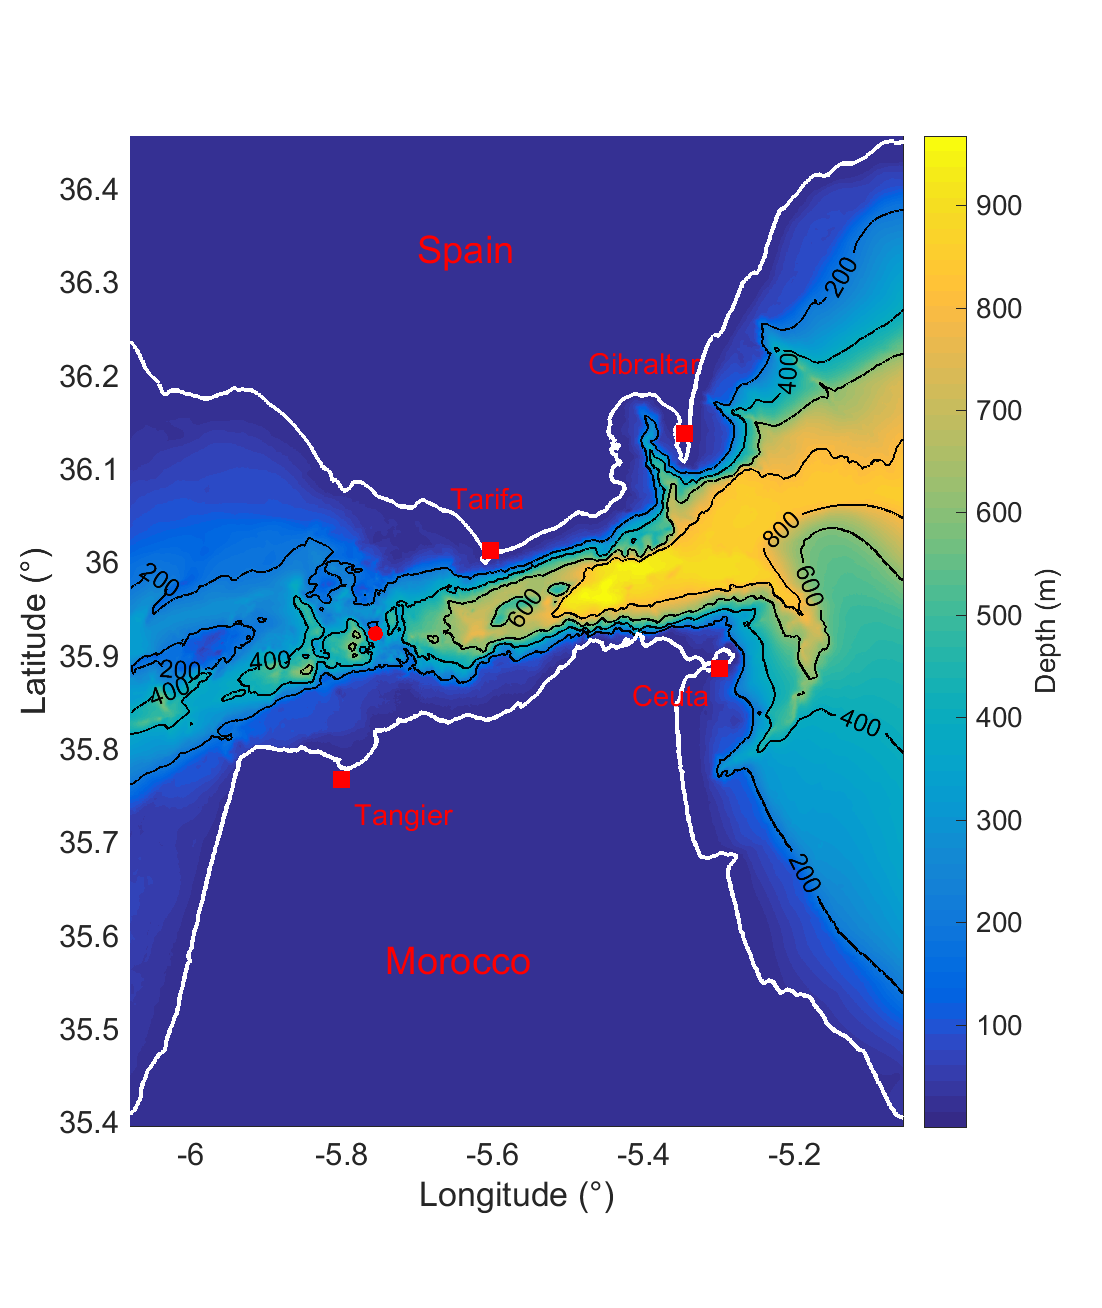
\includegraphics[width=0.5\textwidth]{./GBR3D/FigBathyVHR.png}
        \caption{Area and Bathymetry used for the simulations. The red dot denotes the point at Camarinal Sill where the zonal barotropic current is taken as reference in following figures.  \color{green}Changer en anglais tangier \color{black}}
        \label{FigBathy3D}
\end{figure}

\begin{figure}[!h]
        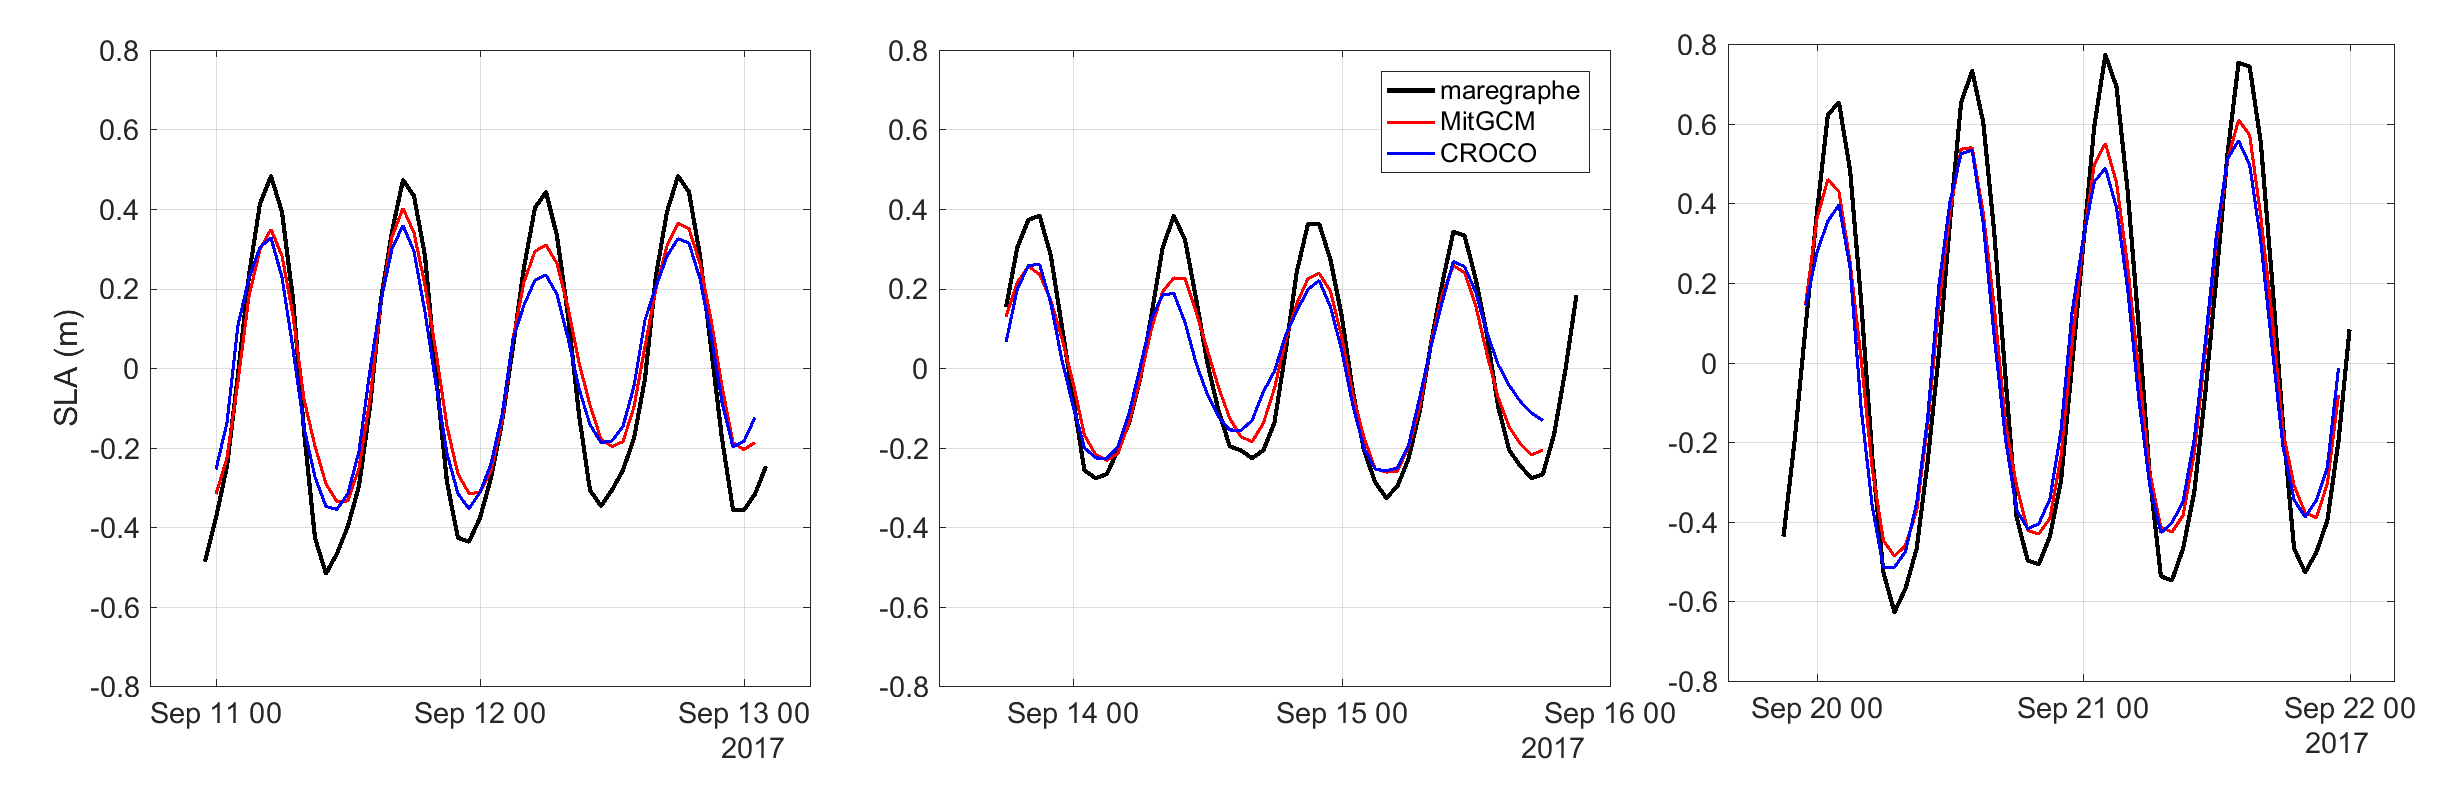
\includegraphics[width=\textwidth]{./GBR3D/SLA_Tarifa_ME2VE2IES.png}
        \caption{Sea level-anomaly at Tarifa: tidal gauge data (black), nearest grid point for parent MitGCM simulation (red) and HR CROCO simulation (blue) during ME (a), MM (b) and VE (c) events.}
        \label{fig_maree_tar}
\end{figure}

\subsubsection{Water masses.}
\label{sectionWaterMasses}
Figure (\noparref{Fig_Ini_WM3D}.A) and (B) show \color{blue} the $\theta-S$ diagrams in the eastern and western parts of the domain \color{black} \sout{entries of the strait} computed for \color{blue}the field of tracers used to initialize the \color{black} simulation SimIT. 
\begin{figure}[!h]
        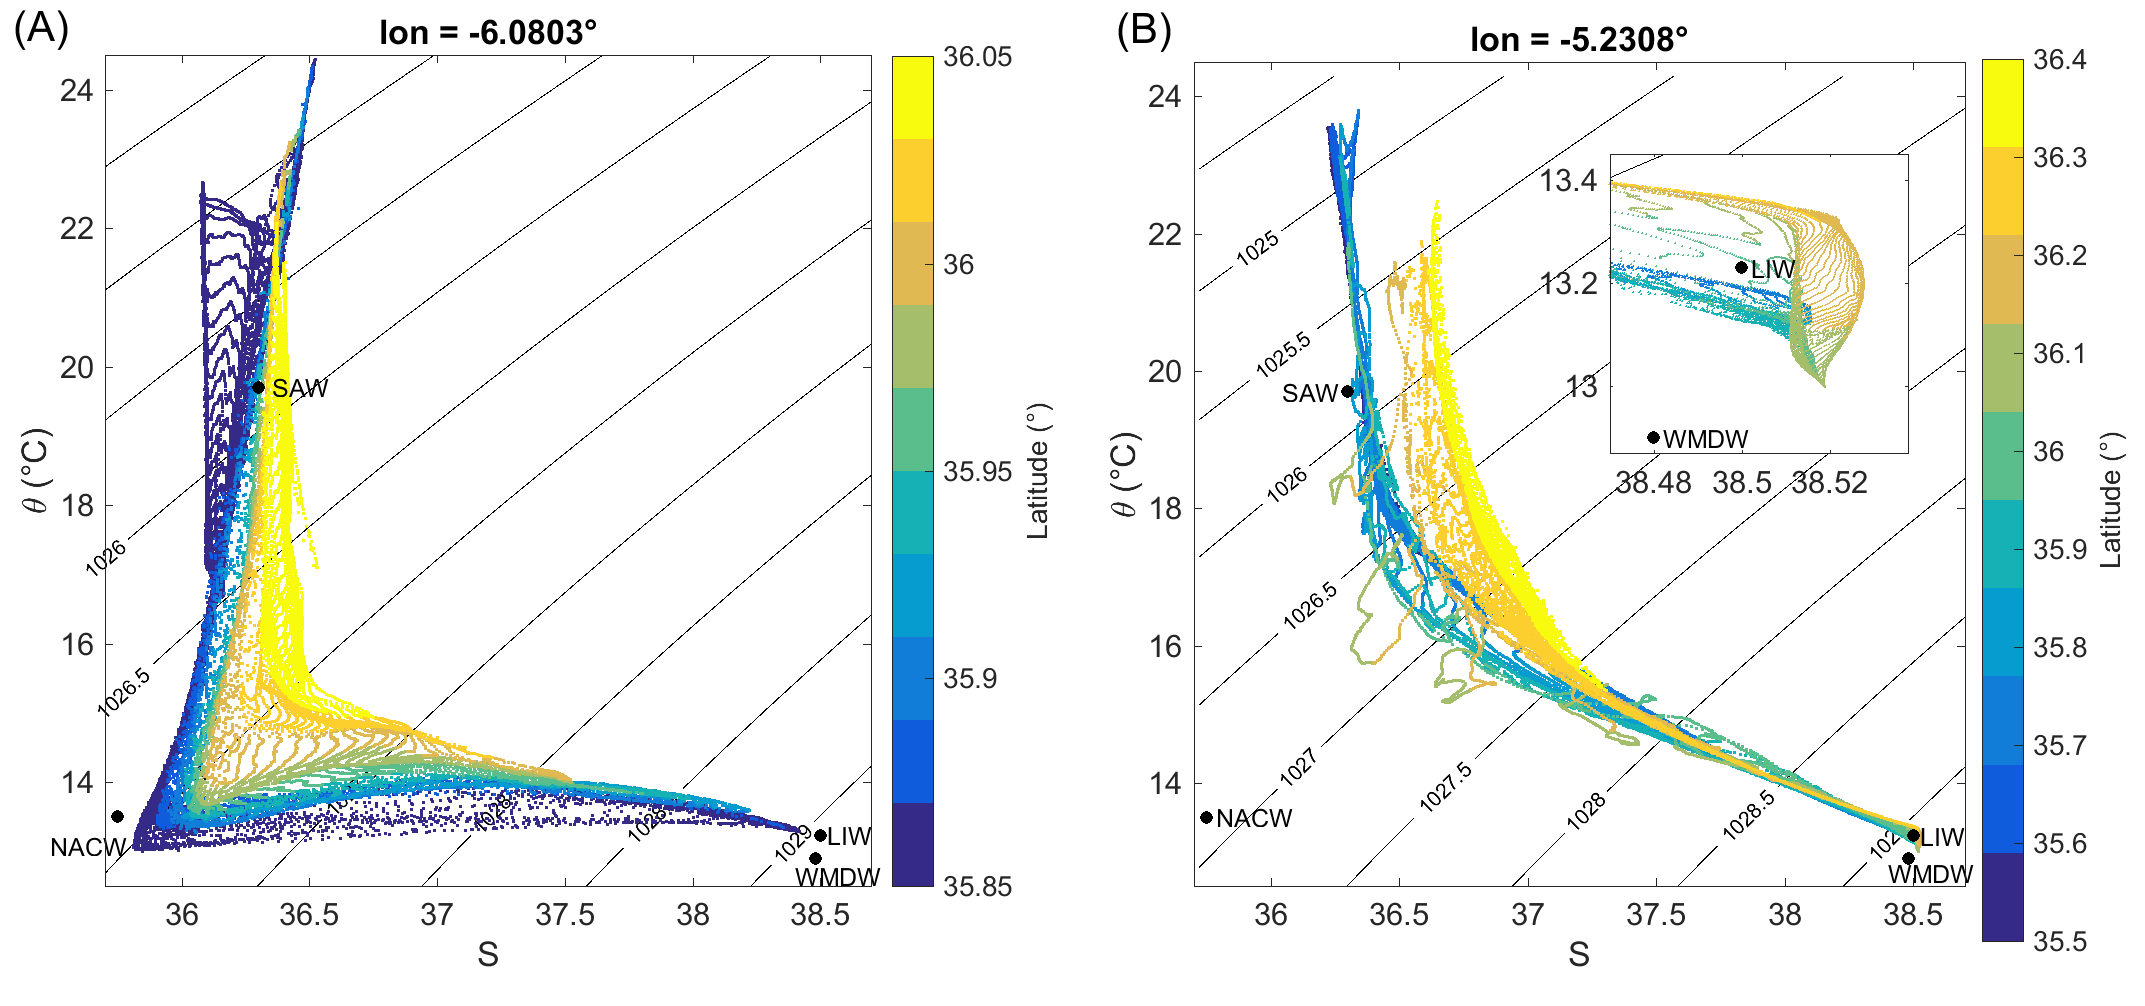
\includegraphics[width=\textwidth]{./GBR3D/WM_ini_IES.png}
        \caption{$\theta$-S diagrams computed at 6.08$^\text{o}$ W (a) and 5.23$^\text{o}$ W at first time step of SimIT. Color indicates the latitude of each grid point. \color{green}Cenroid (???) \color{black}definition of the water masses according to Najanro2014 are also indicated.}
        \label{Fig_Ini_WM3D}
\end{figure}

At the eastern boundary (figure (\noparref{Fig_Ini_WM3D}.B)), the signatures of a deep water mass and of an intermediate water mass that correspond respectively to WMDW and LIW can be identified. The latter is present mostly in the northern part of the domain. The simulated waters are however saltier and warmer than the corresponding water masses observed in the region as per \citet{naranjo_2014}.

At the western boundary now, the signature of two Mediterranean water masses corresponding to the two pathways of the Mediterranean outflow, centered around 35.8°North and 35.9°North, can be identified.
As far as Atlantic waters are concerned, NACW are mostly present on the western part of the domain. 

\color{red}surface waters in the east section have two signals, one nirth, one south, the southern one would correspond to the water directly carried out of the strait bybthe atlantic jet in the simulation\color{black}

%----------------------------------------------------------------------
\subsection{Numerical diagnosis}
%----------------------------------------------------------------------
\label{PartDiag3D}

\subsubsection{Hydraulic control}
\color{green} 
\textit{Il faut introduire ici les raisons pour lesquelles tu as besoin de définir clairement l'interface, ce qui n'est pas évident si tu l'introduis indépendemment de la suite... je te propose donc de regrouper cela dans une section associée au contrôle hydraulique... .} \color{black}\\

\color{blue}The presence of an hydraulic control is probably the most important diagnostic to be carried out in the region of the Gibraltar strait. The exchange flow through the strait can shift from a so-called subcritical to a critical regime in only a few hours. This shift is associated to the occurrence (or not) of an hydraulic jump somewhere in the region of the strait. The bathymetry of the region is characterized by a complex network of pathways for the water masses which implies that hydraulic jump can appear or disappear locally. A consequence is that the classification of the whole strait in one "asymptotic" regime or the other is far from simple and probably not even necessary to explore the dynamics of the region.\color{red}(bof, laisser de côté...fait un peu introduction)

Flow in the Strait of Gibraltar can shift from subcritical to supercritical in only a few hours. Diagnosing the hydraulic control at each instant of the tidal cycle is then a necessity, and must be done locally to account to the complex bathymetry of the region. 

\color{black}

((Diagnostics carried out in the 2D, academic configuration proposed in section {XXX} consequently need to be refined and, in any case, must be local.\\

To start with, "a" local Froude number needs to be computed and,\color{red}meeeehh\color{black} to do so,  the superposition of the Atlantic and Mediterranean water masses (when effective) must be caricatured as a simple two-layer (at most three-layer if one wants to single the interface) representation of the stratification.

In the previous section \ref{sectionWaterMasses}, Atlantic and Mediterranean water masses have been clearly identified based on their signature in temperature and salinity. Salinity is probably the most pertinent tracer to differentiate these waters in the region of the strait due to the large contrast of salinity existing between Mediterranean and Atlantic water masses.
An approximate, local, two-layer analysis can thus be carried in the present, fully-3D , realistic configuration if
\color{black}
\sout{The analysis of simulation result is based on two layer definition of an Atlantic waters layer and Mediterranean waters layer. They are} defined in regard to a reference salinity. In this case, the interface is defined as the height of the first water parcel \sout{from the top down} in the water column for which salinity is above the reference salinity prescribed for Mediterranean waters.

This reference salinity is taken as varying along the strait as a hyperbolic tangent function of longitude centered at CS to account for the different water mass composition in the eastern and western part of the strait of Gibraltar. 

\begin{equation}
	S_i(x)=tanh(\frac{l-L_{CS}}{dl})\frac{S_M-S_m}{2}+\frac{S_M+S_m}{2}
\end{equation}
with $L_{CS}=5.75^o$, $dl=0.25^o$, the location and width of the Camarinal Sill in degrees, $S_M=37.39$ and $S_m=37.1$ the max and minimum interface values taken respectively east and west of the sill.

With the Atlantic and Mediterranean layers defined above, the Froude layer number for internal gravity waves is computed for \color{blue} a given water column as\color{black}: 

\begin{equation}
F_i=\frac{U_i^2}{g'h_i} , \ \text{with} g'=g \frac{\rho_2-\rho_1}{\rho_0}
\end{equation}
where $\rho_i$ averaged density in layer i,  $U$ is averaged velocity norm over the layer i of height h. $F_i>1$ means that the flow in layer i is supercritical.


\subsubsection{Hydraulic jump detection, acceleration of flow}
\color{blue}The necessity not only to caricature the stratification but also to evaluate a local phase velocity of internal waves based on this stratification renders the evaluation of a local Froude number rather complex and, as a consequence, can somehow blur the characterization of the local regime of the dynamics.  \color{black}
Another simple diagnosis for detection of the hydraulic jump at Camarinal Sill in the simulations is \color{black} proposed based \color{black} on the impact such a structure is known to have on the flow. 
\begin{figure}[!h]
 \centering
 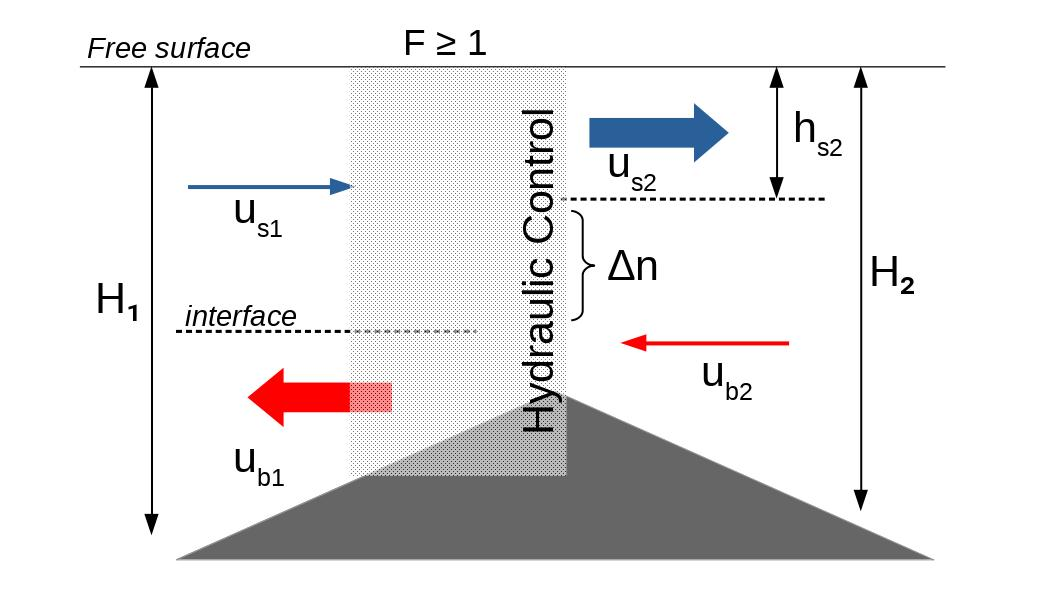
\includegraphics[width=0.5\textwidth]{./GBR3D/schema_diagressaut.jpg}
 \caption {Schematic of flow upstrean and downstream of hydraulic jump at Camarinal Sill in the Strait of Gibraltar.}
  \label{schemaRH}
\end{figure}
As schematized on figure \ref{schemaRH}, an hydraulic jump (also called hydraulic drop) induces a drop of the interface depth. Since the flow in the Strait is \color{blue}channeled \color{black} by the bathymetry (for the Mediterranean flow at least) and the coast (for the Atlantic flow), there must be conservation of the flux from \color{blue} a downstream section to an upstream section \color{black} of the hydraulic jump. The variation of the interface depth is indeed associated to an acceleration or a deceleration of the flow (depending on which layer is \color{blue}chosen as a \color{black}reference).
\color{green}Je pense qu'il faut changer les notations et conserver plutôt $h_*$ pour les épaisseurs plutôt que b, notation souvent utilisée pour la flottabilité et n pour une numération entière." \color{black}
The drop in the interface depth is noted $\Delta n=b_2-b_1$, the variation of bottom depth $\Delta H=H_2-H_1$ and the acceleration in the bottom layer $\Delta u_b = u_2-u_1$. In the bottom layer, the conservation of the flux leads to:
\begin{subequations}
\begin{alignat}{2}
  \displaystyle
&u_1 (H_1-b_1)&& = u_2 (H_2-b_2)\\
& &&= u_1 (\Delta H + \Delta n) + u_1 (H_1-b_1) + \Delta u_b (H_2-b_2)
\end{alignat}
\end{subequations}

\begin{equation}
\Delta u_b = -u_1 \frac{\Delta H + \Delta n}{H_2-b_2}
\end{equation}

For the surface flow:
\begin{equation}
\Delta u_s = - u_1\frac{\Delta n}{b_2}
\end{equation}

The velocity in the area of the hydraulic jump must validate the condition of (at least) critical flow, i.e. Froude number $\geq$ 1 at the shallower location. A minimal condition for hydraulic jump is consequently $F\ =\ 1$, or $U\ =\ c$: the flow velocity must be equal to the local phase speed of internal waves. If, for the latter, \color{blue} an expression for $u_1$ is given by the definition of interfacial velocity  \color{green}(is this what you mean?): \color{blue} 
\begin{equation}
|u_1|=c=\sqrt{g' \frac{(H_1-\Delta n - b_2)(\Delta n + b_2)}{H_1}}
\end{equation}
 \color{green}Il faut que tu reformules et que tu expliques un peu plus ce qui suit... difficilement reproductible par un lecteur qui découvre ce diagnostique. Tu peux ajouter une petite explication en annexe si tu as peur que cela fasse trop dans la partie principale. \color{black} 
Several parameters are chosen as threshold, here take values that should be correct for area of camarinal sill, the minimum excursion of the jump $\Delta n = 30m$ and the height of the Atl layer $b_2=50 m$ , and the reduced gravity $g'\ =0.02\ m.s^{-2}$.

\subsubsection{Q parameter and derivated diagnosis}

\color{blue}The studied configurations are all based on grid resolutions of a few tenths of meters, an objective being the explicit simulation of at least the largest turbulent eddies. The region of the Mediterranean outflow is of particular interest since large velocity shears are known to be associated there to a large vertical density (salinity) stratification. This region is thus a key area to better understand and simulate the mixing of Mediterranean and Atlantic water masses in Gibraltar strait.\\
A dedicated diagnostic is now proposed to "detect" the primary instabilities and more specifically to identify Kelvin-Helmholtz instabilities developing potentially in this region. \color{black}
\color{blue} A careful inspection of the relative-vorticity vector can fulfill this purpose and a dedicated scalar diagnostic based on the components of this relative vorticity is retained. It is a generalization of the Okubo-Weiss parameter retained in Hilt (2020) to the present 3D realistic configurations. \color{black}
%A simple vorticity diagnosis is not chosen as it requires choosing the rotation axis, but also because regions of high shear such as between the MEd outflow and Atl waters will have high vorticity values. Instead, analogously to the use of the Okubo-Weiss parameter in Hilt 2020, we chose to compute parameter Q, defined as (ref):
\begin{equation}
Q=-\frac{1}{2} \frac{\partial u_i}{\partial x_j} \frac{\partial u_j}{\partial x_i} = \frac{1}{2} (\Omega_{ij}\Omega_{ij} - S_{ij} S_{ij})
\end{equation}
with $u_i$ the components of velocity vector, and $S_{ij}$ and $\Omega_{ij}$ are respectively the strain-rate tensor and vorticity tensor. When $Q\ >\ 0$, rotation is larger than shear.
\color{green}Attention à la cohérence des notations ui etc... tout au long du manuscrit. $\Omega$ est en particulier déjà utilisé pour la rotation de la terre, $\omega$ est plus courant pour la vorticité relative.\color{black}\\

\color{green} Beaucoup trop tôt je pense pour le paragraphe suivant... A ce stade, tu introduis tes diag et éventuellement approches statistiques rendues nécessaires par les configurations auxquelles tu t'attaques. Place-toi si possible dans un cadre un peu plus général. Tu peux déplacer le paragraphe suivant. \color{black}
\sout{Due to advection by the Med outflow, a succession of primary instabilities \sout{will} propagate over the same grid cells.} The temporal evolution of Q over such grid cells show \color{green}(évite l'utilisation du futur) \color{blue} oscillations between high positive values (at the center of a billow or a vortex for instance) and low negative values (sheared layers between two consecutive billows for instance). A "proxy" to detect this area is the maxima or at least the largest values of the standard deviation of parameter Q. This proxy is defined in equation \ref{eqstdQ} where the overbar denotes temporal average over 30 mn, a time-scale considered here as smaller than the time-scales of the dynamical structures the present study is interested in.\sout{a period over which there will be minimal modification of the general flow in the strait}. \color{black}

  \color{green}\begin{equation} 
\label{eqstdQ} 
    std ( Q ) (\vec{x},t)=  \sqrt{   \overline{Q (\vec{x},t)^{2}} -  \overline{Q(\vec{x},t)}^{2}  }
\end{equation}

 \color{blue}\begin{equation} 
\label{eqstdQ} 
    std ( Q ) (\mathbf{x},\ t)=  \sqrt{   \overline{Q (\mathbf{x},\ t)^{2}} -  \overline{Q(\mathbf{x},\ t)}^{2}  }
\end{equation}
 \color{green}Sur les conseils des rapporteurs des différents papiers que nous avons soumis ces derniers temps... je pense qu'il est salutaire d'abandonner les notations vecteurs avec des flèches dans nos écrits en les remplaçant par l'utilisation des caractères gras... Nous en rediscuterons à l'occasion si tu veux. \color{black}

To create the 2D maps presented in the following section, only the maximal value of standard deviation in the water column \color{blue}needs to be saved.
By implementing this calculation online in CROCO, we can asses where instabilities or vortexes propagate without having to make a huge volume of simulation outputs over the whole domain, thus economizing storage and data readability. \color{black}
The result of this proxy can be compared to the result of the Singular Value Decomposition (SVD) of the time-varying 3D field.  \sout{C'est peut-être ici qu'il faut donner quelques explications sur cette SVD. Je t'assure qu'un lecteur extérieur ne comprendra absolument pas où nous voulons en venir. Du coup ce que je peux te conseiller est de consacrer un petit paragraphe ou une sub-section à cette SVD: pourquoi (besoin)? comment ? apport ? S'il se révèle nécessaire de donner quelques explications mathématiques spécifiques à ton utilisation, je pense que cela peut être fait en annexe. Lucie s'était résolue à le faire si je me souviens bien, je pense que tu peux trouver cela dans son manuscrit.} \color{black}
 \color{blue}SVD computations requires a priori the storage of the field to be decomposed. This could not be made online: SVD have consequently been computed off-line which necessitates high frequency 3D outputs to pick up the relevant structures. \color{black}

%----------------------------------------------------------------------
\subsection{Fine scales in the strait of Gilbraltar}
%----------------------------------------------------------------------
\label{section3DRes}

\subsubsection{Flow criticality/Hydraulically controlled layer and hydraulic jump, neap-spring tide variability}
\label{section3DResFlow}

\begin{figure}[!h]
 \centering
 
 \begin{subfigure}{\linewidth}
\centering
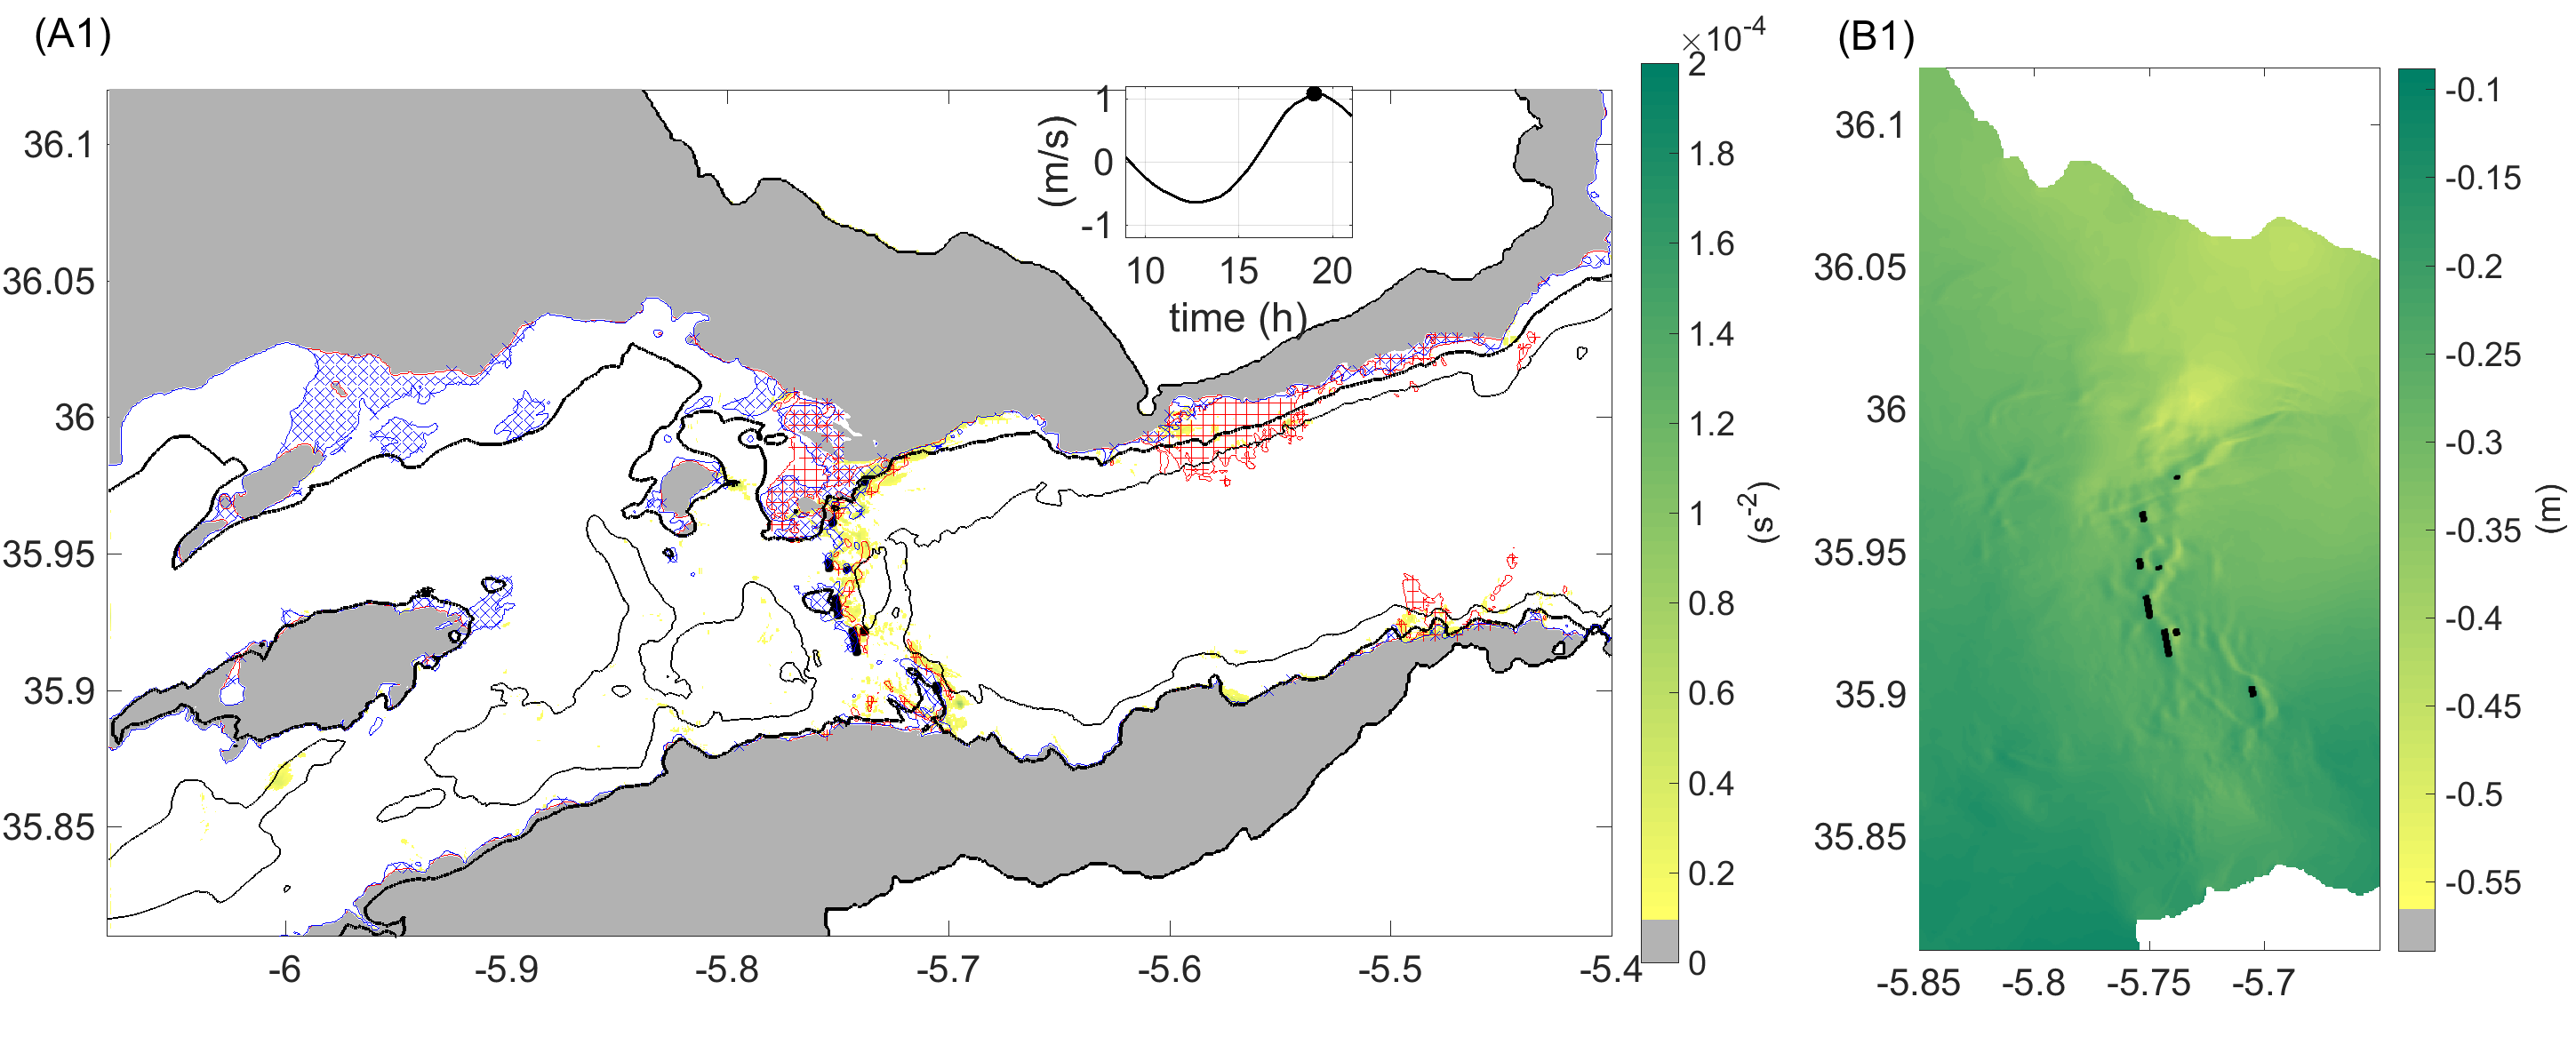
\includegraphics[width=1\linewidth]{./GBR3D/ME2_19h_p.png}
\end{subfigure}
 
 \begin{subfigure}{\linewidth}
\centering
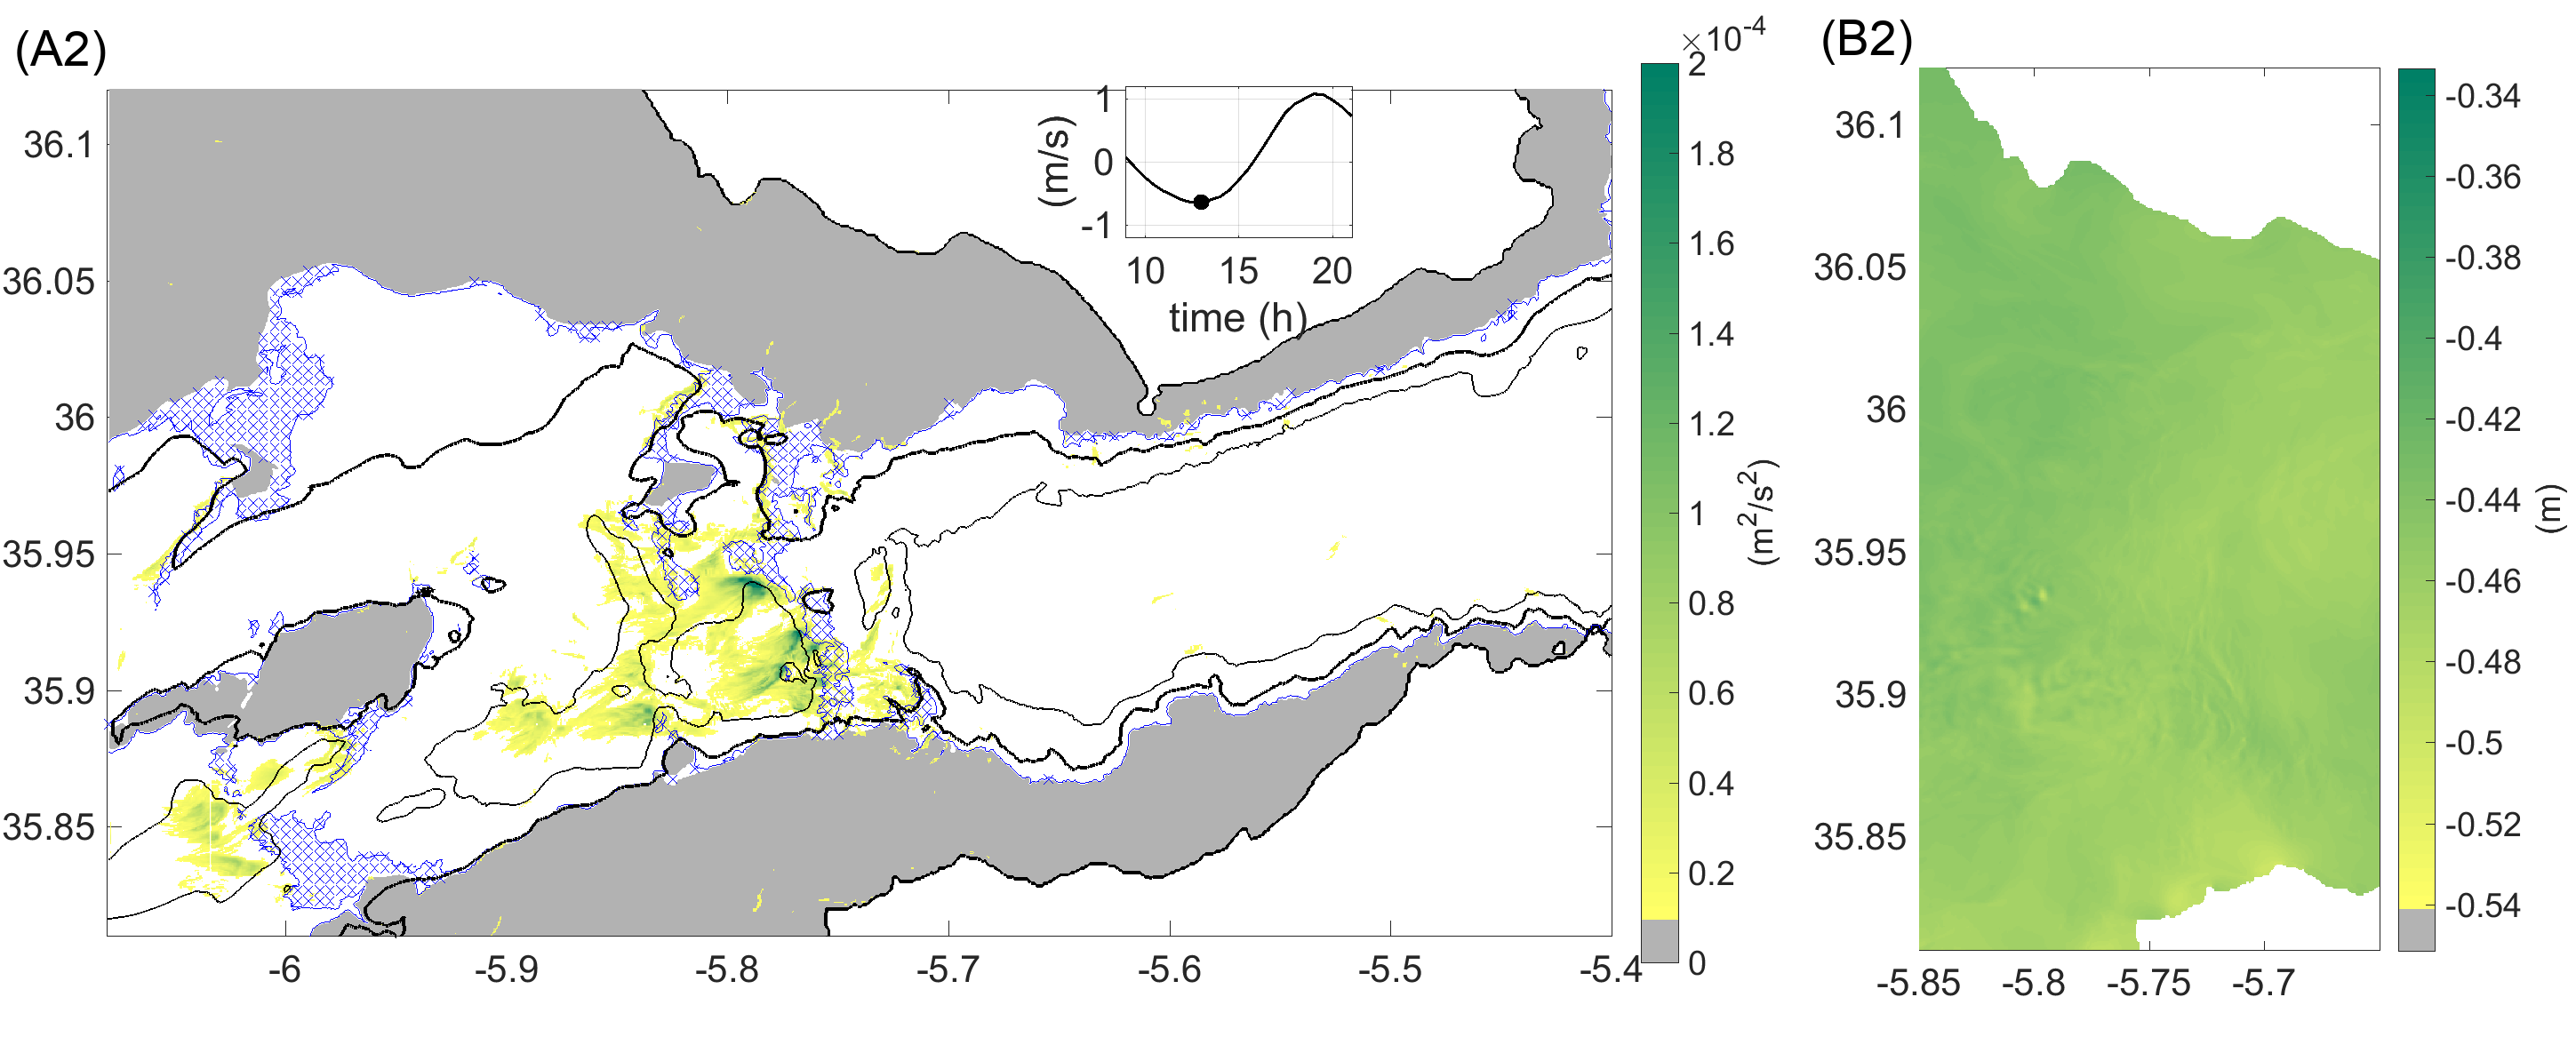
\includegraphics[width=\linewidth]{./GBR3D/ME2_13h_p.png}
\end{subfigure}
\caption { \color{blue} \sout{For simulation SimNT} consecutive inflow and outflow in configuration SimNT, \textit{no-jump} case. The blue (red) shaded areas correspond to supercritical Mediterranean (Atlantic) layers. Black dots show locations where an hydraulic jump has been detection (\S XXX). The grey areas denote where $S_{bottom}\ <\ S_{interface}$ respectively the salinities at the bottom and at the interface between the two water masses. Colorbar is related to the standard deviation of parameter Q (only values above $10^-5$ are represented). Barotropic zonal currents at CS (point indicated in figure \ref{FigBathy3D} are also indicated). Two black isobathes contours are shown: 200 m (bold) and 400 m (thin). \color{green} Oups, cette légende demandait une grosse ré-écriture! \color{black}}

\label{FigHCN}
\end{figure}

Figures \ref{FigHCN} to \ref{FigHCI} present several diagnosis for a series of maximal outflows and inflows \color{blue} with \color{black} variable strength of the tidal forcing in configurations SimNT, SimST and then SimIT \color{blue}Table (XXX) \color{black}. The corresponding diagnosis are presented in paragraph \ref{PartDiag3D}: \color{blue}the shaded regions correspond to areas of supercritical flows (\S XXX) in either the Atlantic or Mediterranean layers. On top of these shaded regions, the locations of hydraulic jumps are indicated (\S XXX) together with the areas of large standard deviations of parameter Q (\S XXX) (potentially associated to propagating primary turbulent eddies). \color{black} The grey area indicates where the salinity in the bottom level is below the interfacial salinity as defined in \S XXX, and thus \color{blue} where Atlantic waters are exclusively present in the water column. \color{black}

Figure \ref{FigHCN} presents a \color{blue} neap-tide situation \color{black} of weak barotropic currents ($\ <\ 1\ m/s$ at a shallow point of CS) in \color{blue} both outflow and inflow conditions\color{black}. Figure \ref{FigHCS} \color{blue} corresponds to \color{black} strong barotropic currents ($\geq 1.5\ m/s$) in inflow and outflow conditions during a spring-tide period. Finally, figure \ref{FigHCI} corresponds to a period of outflow with intermediate-strength ($\approx 1\ m/s$) of the barotropic currents. \color{black}

\begin{figure}[!h]
 \centering
\begin{subfigure}{\linewidth}
\centering
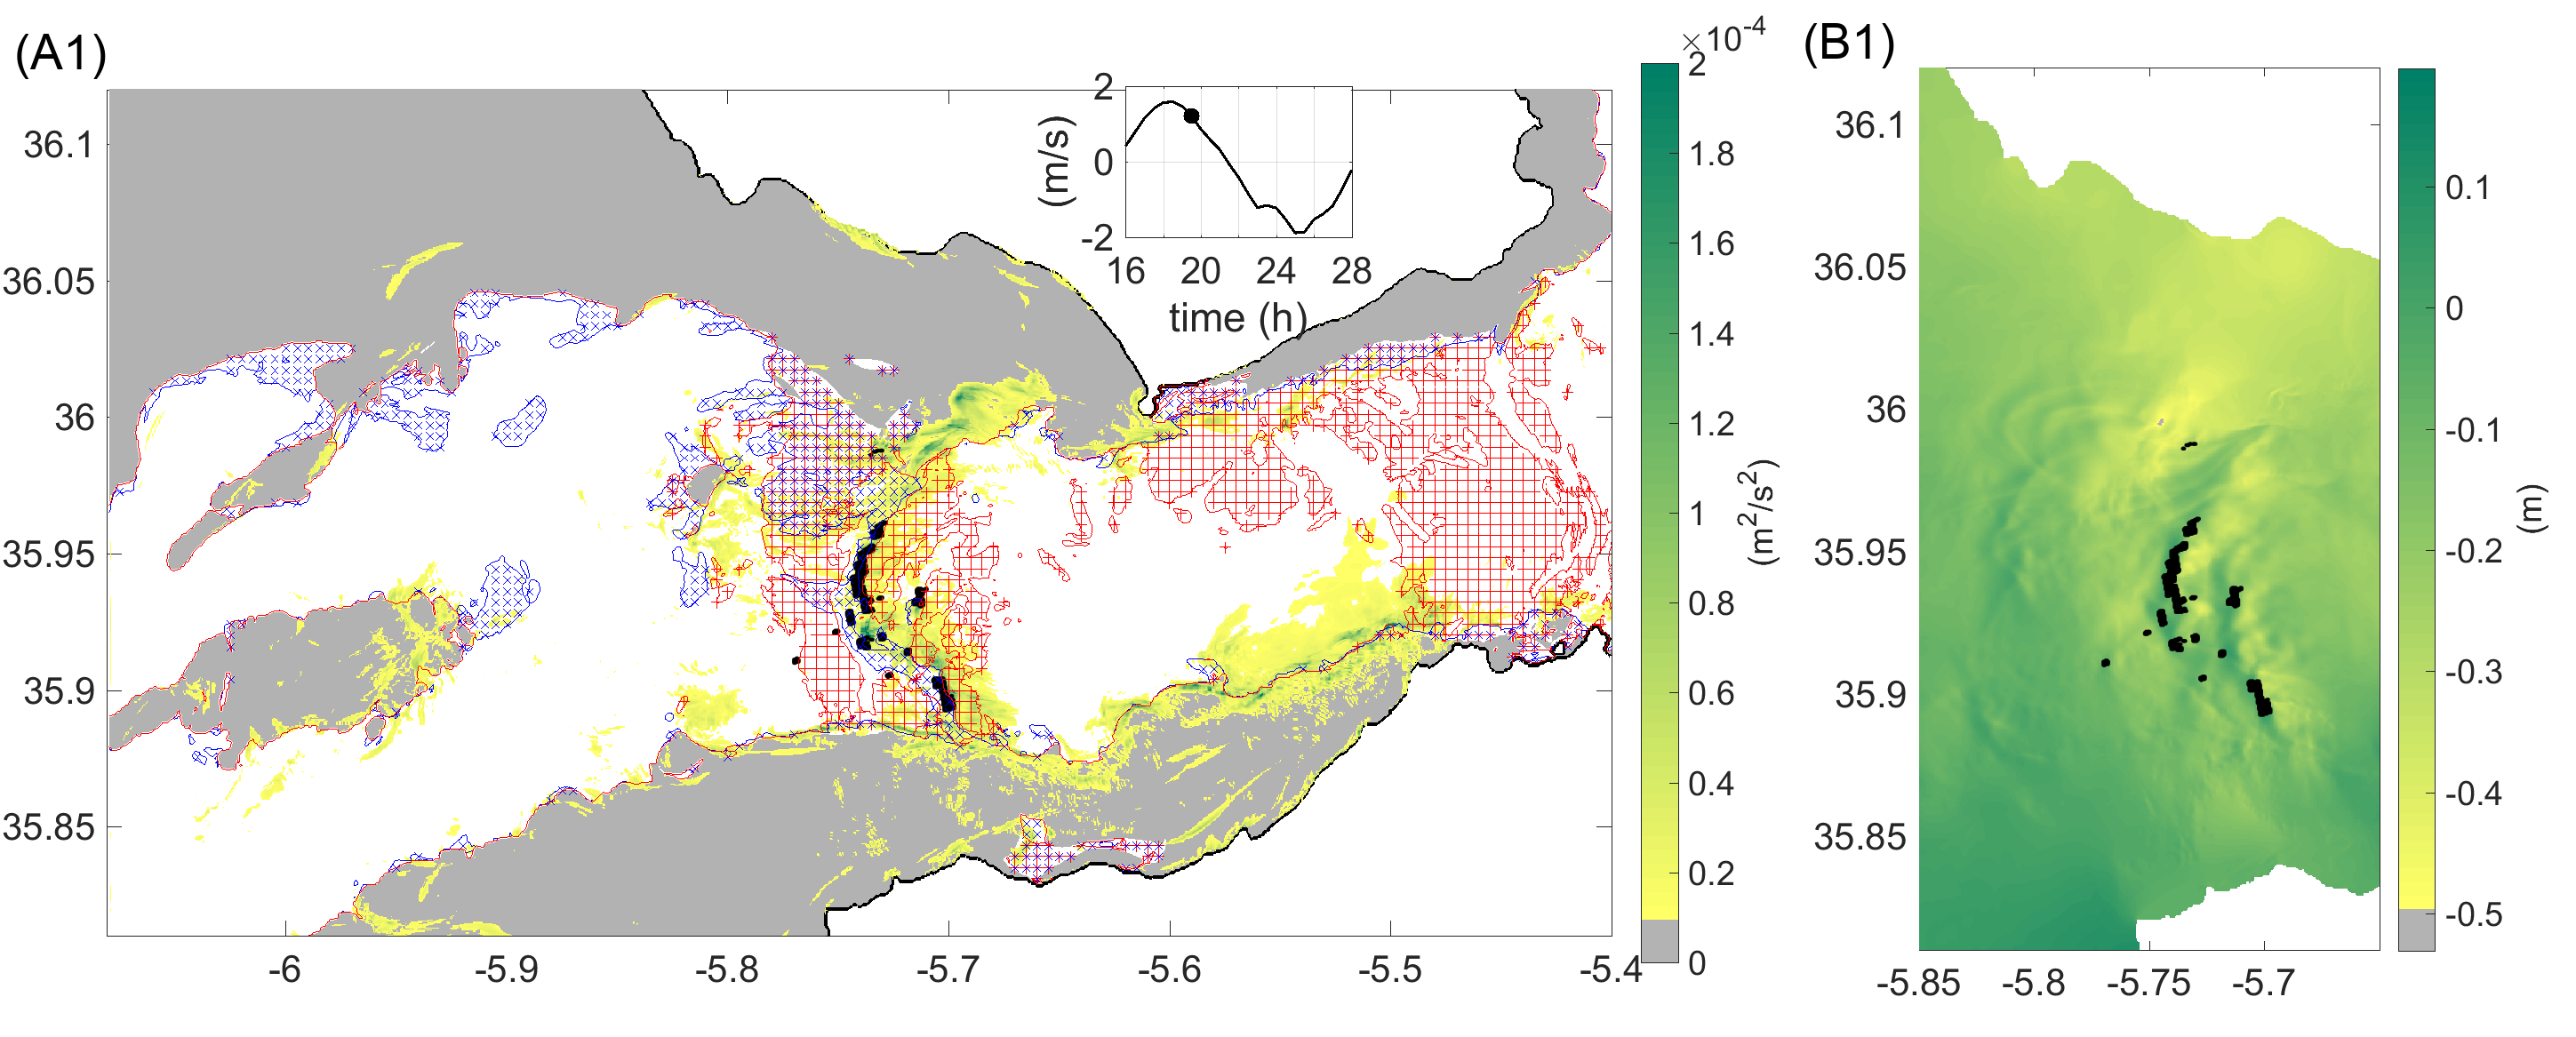
\includegraphics[width=\linewidth]{./GBR3D/VE2_19h30_p.png}
\end{subfigure}

\begin{subfigure}{\linewidth}
\centering
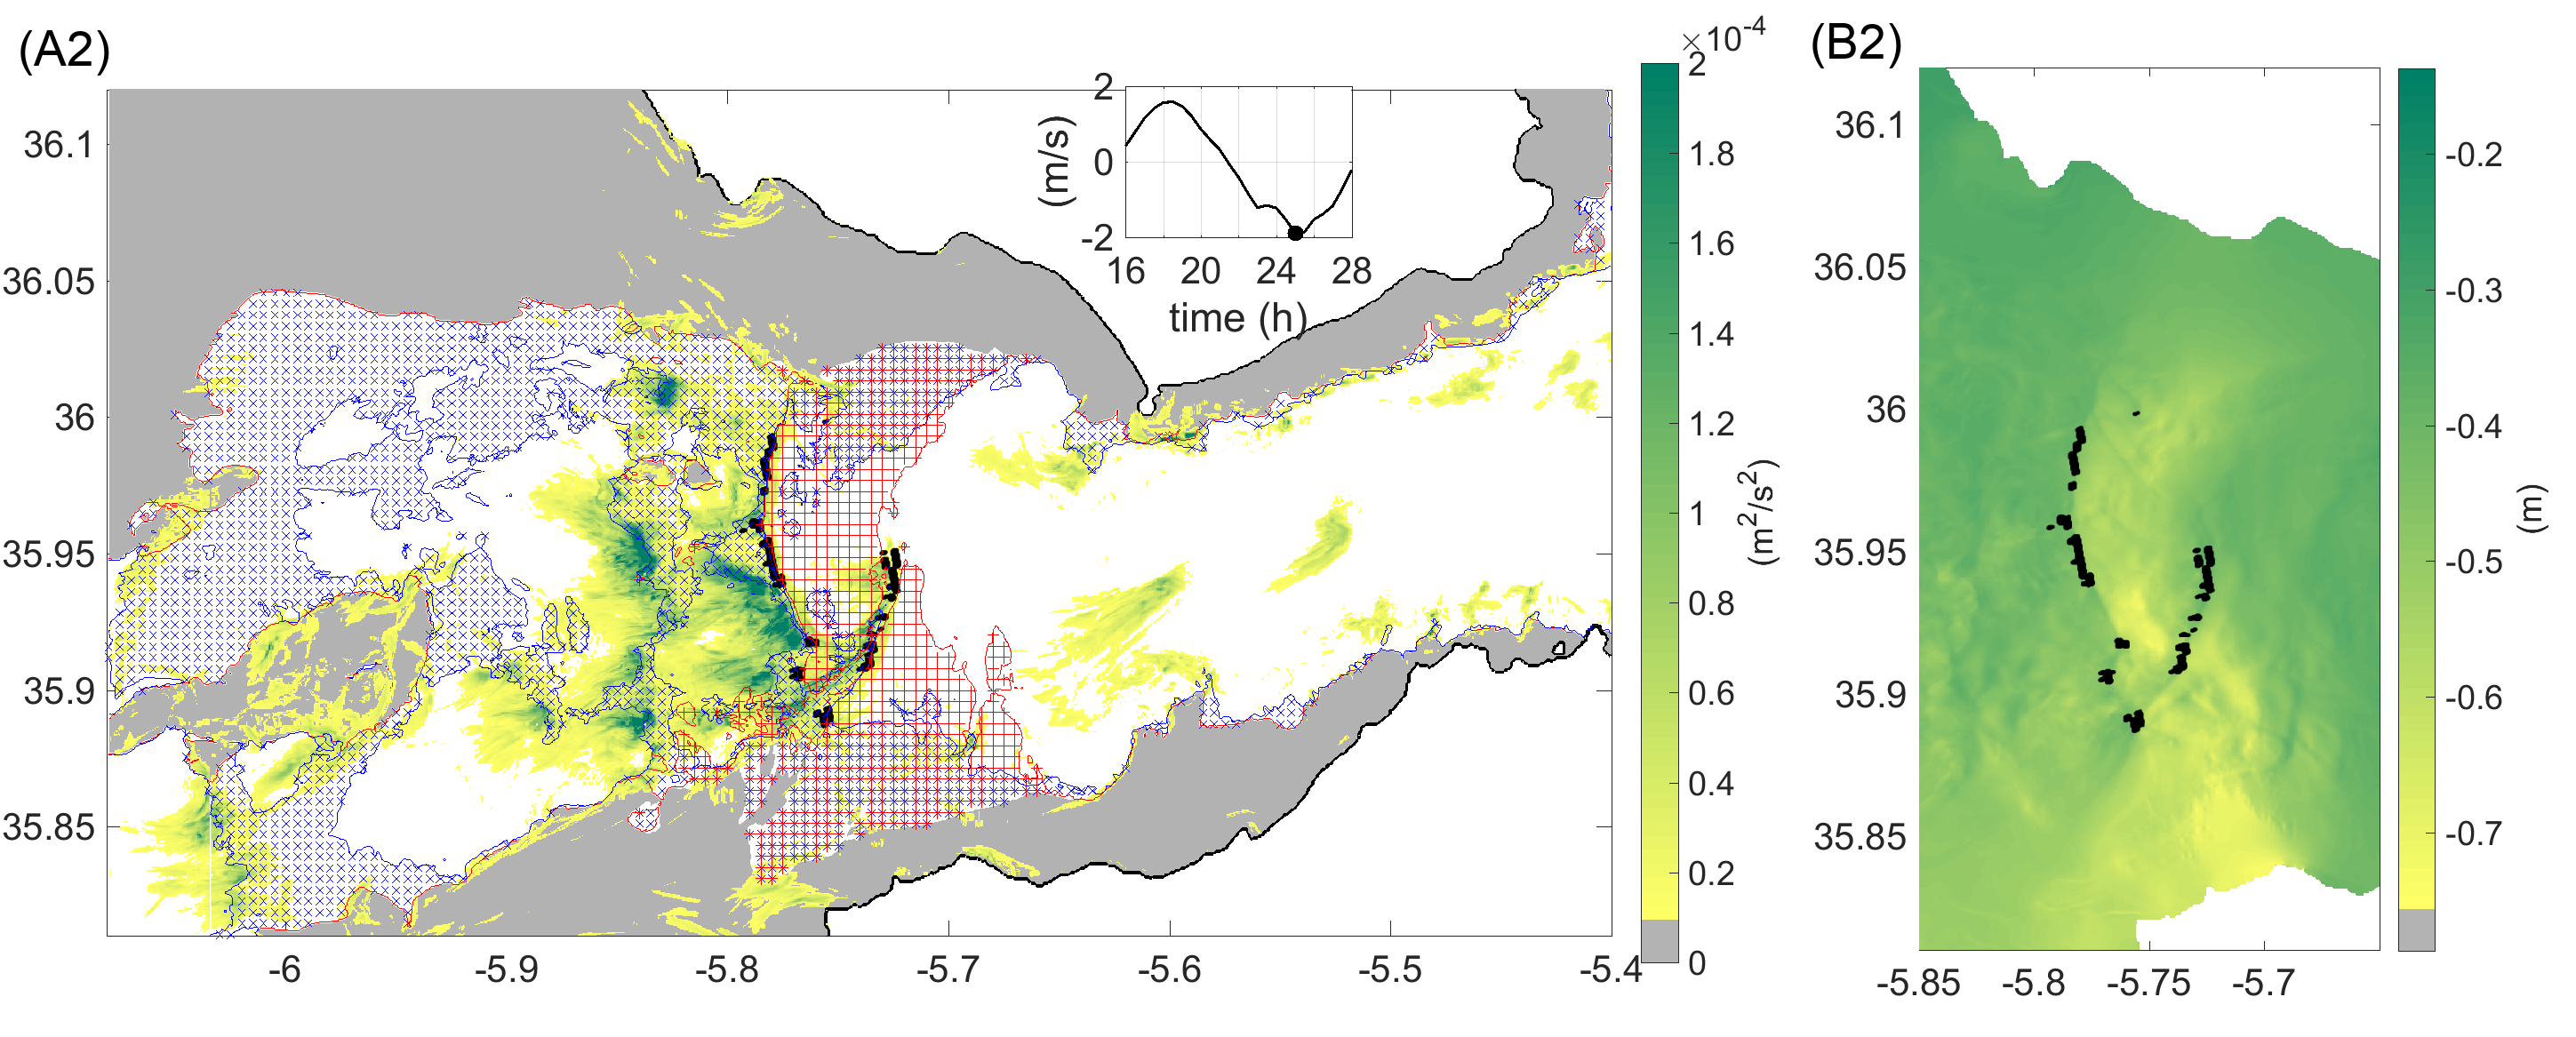
\includegraphics[width=\linewidth]{./GBR3D/VE2_25h_p.png}
\end{subfigure}
\caption {Same as figure \ref{FigHCN} but for simulation SimST in inflow and outflow of type \textit{w-jump}}
\label{FigHCS}
\end{figure}

\begin{figure}[!h]
 \centering
%\begin{subfigure}{\linewidth}
%\centering
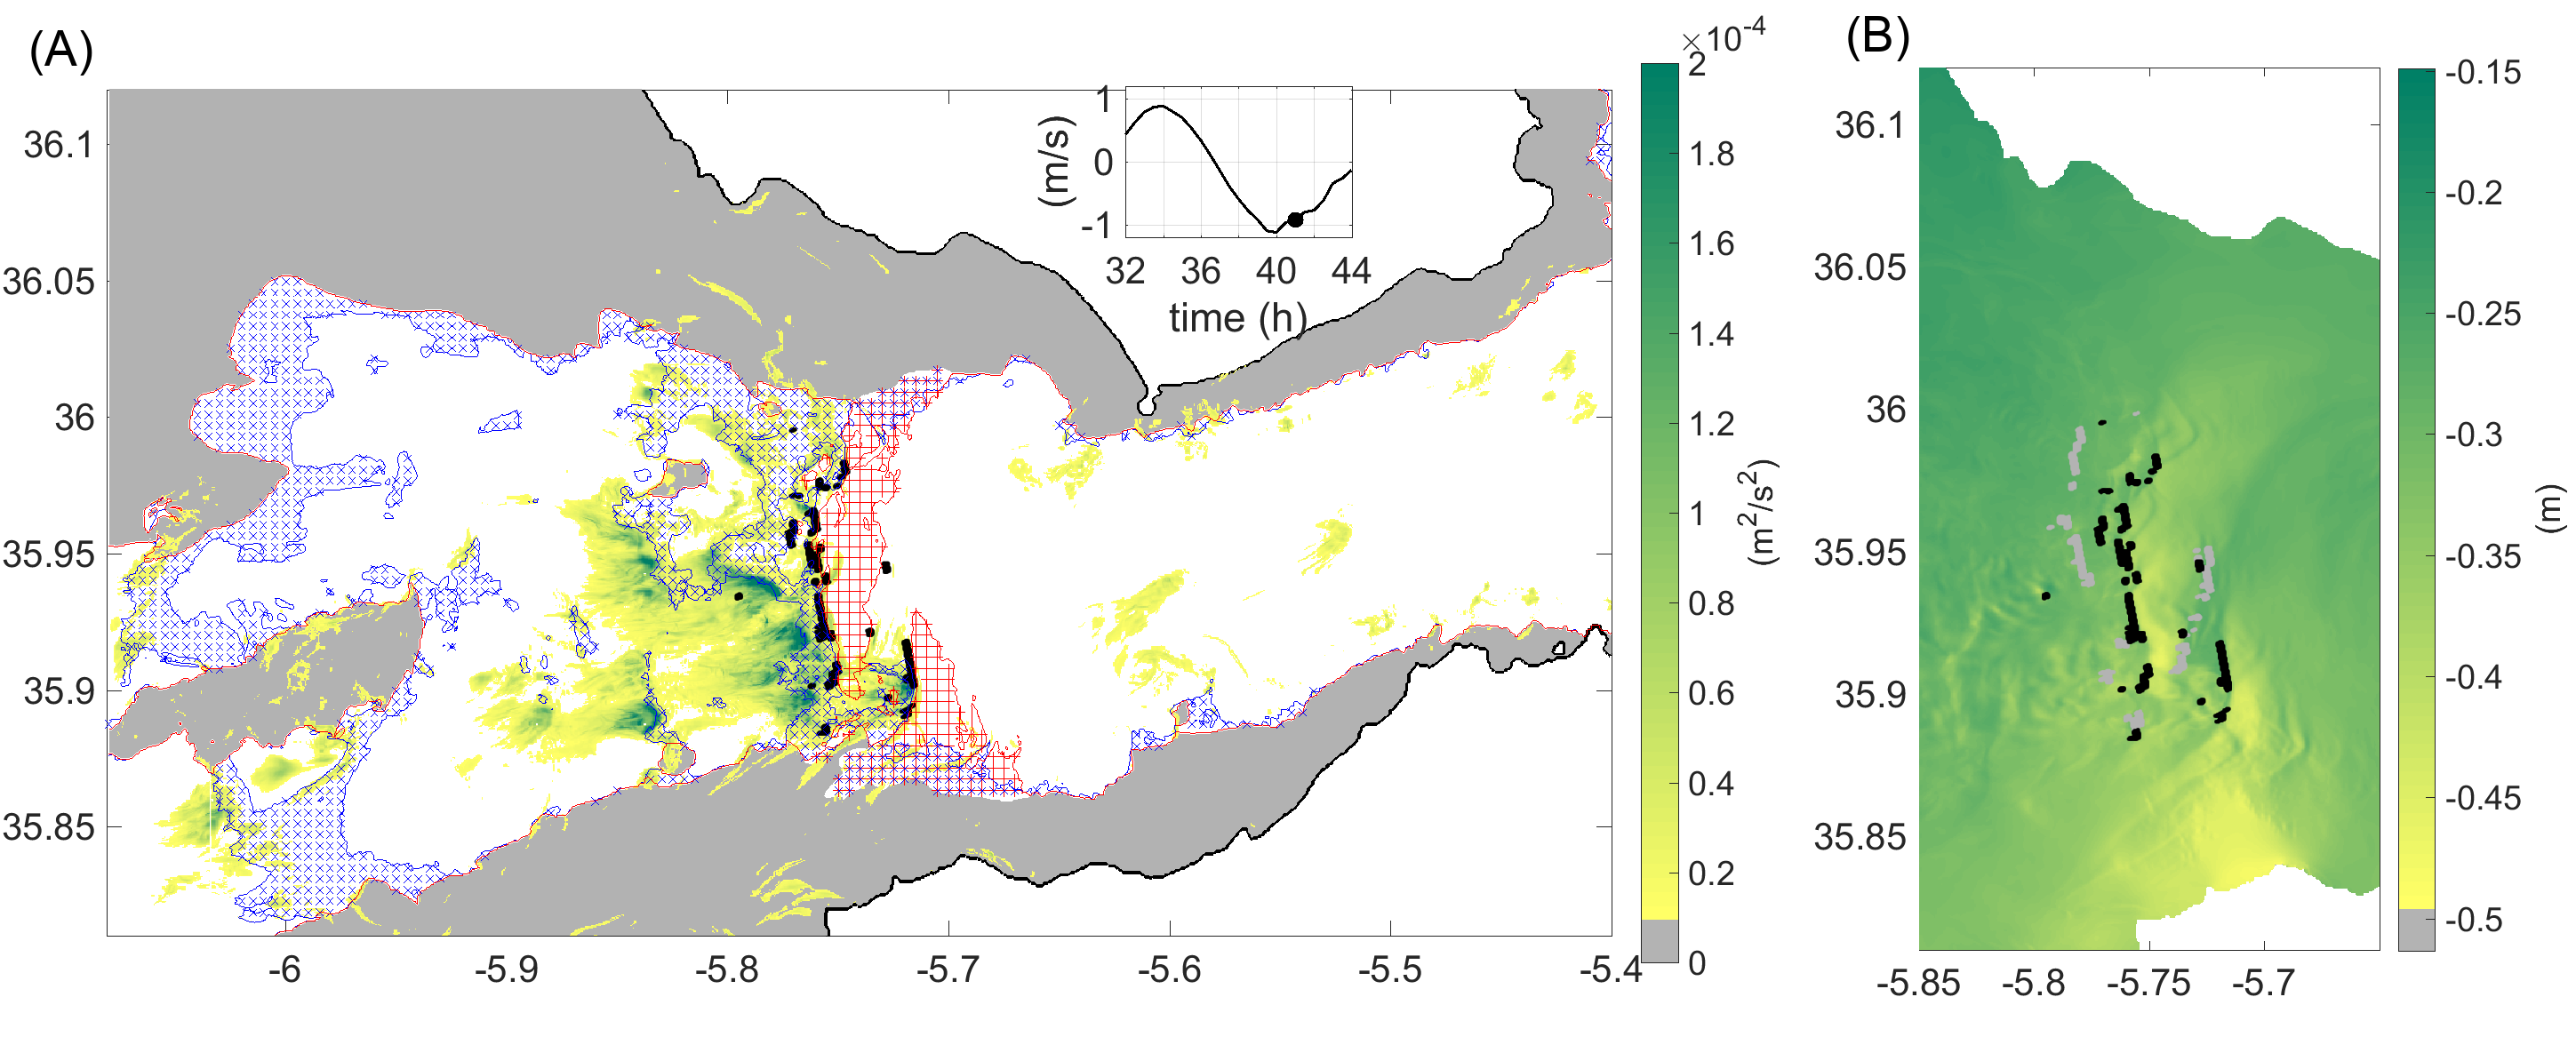
\includegraphics[width=\linewidth]{./GBR3D/IES_41h_p.png}
%\end{subfigure}
 \caption {Same as figure  \ref{FigHCN} but for simulation SimIT and an outflow of type {s-jump}. The sea surface anomaly (SLA) shows the signature of the hydraulic jump of spring tide outflow}
 \label{FigHCI}
\end{figure}

\color{green}Attention, tu as laissé beaucoup de formulations sans verbe de ce type: 
\sout{Firstly, can see two channels west of the Camarinal Sill where Med layer is present, separated by Majuan Bank.} ???\color{black}
\color{blue}Firstly, two veins of Mediterranean water separated by Majuan ban can be found west of CS.
 \sout{The southern vein does not change much, however in the northern channel see a variable area of circulation for med waters above 200m depth and centered at 36$^\text{o}$ N.} \color{green}Reformule lorsque pas de sujet... la tournure me semble peu usuelle en anglais ? Une proposition suit:\\
 \color{blue}
The southern vein does not change much, however, in the northern channel, a  \sout{variable}  \color{green} (What do you mean by variable ? Inhomogeneous ? )\color{blue}  \sout{area of circulation} a pathway for Mediterranean flow can be found above a depth of 200 m, this vein is roughly centered at 36$^\text{o}$ N. \color{black}

This pathway (???) is larger during outflows, as Mediterranean waters are driven up-slope by the westward barotropic current, but \color{blue} the flow presents an additional \color{black} southern component that bends back into the main northern channel (see figure \ref{FigBathy3D} for a better view of the bathymetry of this area).

For all cases, \color{blue} supercritical areas \color{black} of the Atlantic (Mediterranean) layer \color{blue} can be found \color{black} mostly east (west) of 5.8 $^\text{o}$ W which corresponds the western slope of CS. During inflows in figure  \color{blue}(\noparref{FigHCN}.a) and (\noparref{FigHCS}.a), the Mediterranean layer becomes supercritical over several regions (patches are observed): the most extended one in the area of the northern channel has been discussed above. In outflows in Figures (\noparref{FigHCN}.b), (\noparref{FigHCS}.b) \color{green} Je t'ai reformulé qq citations du type 4.a, je te laisse les éventuelles suivantes que je n'aurais pas trouvées...) \color{black} and \ref{FigHCI} the Mediterranean layer is supercritical at both Camarinal and Espartel sills and in the northern channel in all flow cases.  \color{blue}During the spring tide outflow period, most of the northern channel presents a supercritical flow while over ES, there is not much difference between the intermediate and spring tide outflow periods\color{black}.

\color{blue}During the outflow period, the Atlantic layer is supercritical only at CS, except during the neap tide period. When both the Mediterranean and Atlantic layers are supercritical at CS, an hydraulic jump is detected. It is located at the intersection of areas where Atlantic and Mediterranean layers are supercritical. This configuration leads to an area of high gradients of free-surface elevation displacement. Among the simulated tidal cycles, three types of flows can be encountered at CS during the outflow period: (i) no hydraulic jump is located right above the sill (figure \noparref{FigHCI}, \textit{s-jump}),  \color{green} (ii) a disparu ? ma faute? \color{black} and (iii) one hydraulic jump located over the western slope of CS (figure \noparref{FigHCS}.b, \textit{w-jump}). In this latter case, the hydraulic jump actually develops \color{black} over the sill's crest as in the \textit{s-jump} case but since the tidal currents strengthen, \color{blue} an area of supercritical flow develops in the western part of the Atlantic layer and so does the junction (???) where an hydraulic jump can be observed.\color{black} 

\color{blue}An hydraulic jump appears also during inflows, it remains in the same area over the east slope of CS regardless of the strength of tidal currents. It is more pronounced when barotropic currents are stronger, during the transition of flow just upstream of the area of supercritical Atlantic layer. \color{black}

East of CS, another area of supercritical Atlantic layer appears during inflows.  \color{blue}During neap-tide, \color{black} it takes the appearance of a patch near the north shore in TN at 5.59$^o$ W. During spring tide, this patch extends over a larger area. A secondary area of supercritical Atlantic flow exists between 5.5$^o$ W and 5.4$^o$ W, extending from the northern to the southern side of TN. \color{black} 

Figure \ref{FigISWGBR3D} shows \color{blue} the divergence of surface currents in TN while a train of ISW is propagating. Figure (\noparref{FigISWGBR3D}.a) corresponds to a barotropic current of intermediate strength during inflow and figure (\noparref{FigISWGBR3D}.b) to a strong barotropic current during the same period (like figure \ref{FigHCS}.b). The areas of critical Atlantic layer flow are also shown as a black meshed area. The ISW train propagates during the same period with the maximum inflow in this area. \color{green} In the area of critical Atlantic layer is located \color{black} west of the propagating wave train. (je crois que je ne comprends pas où tu veux en venir?)\color{blue} The northern part of the critical area of the Atlantic layer seems to be dissociated from its southern part. The former occurs more often and its extension varies  \sout{while} whereas the latter may be modified by the arrival of the ISWs. This can be due either to the induced velocity or to the change of stratification.\color{black}

\begin{figure}[!h]
 \centering
%\begin{subfigure}{\linewidth}
%\centering
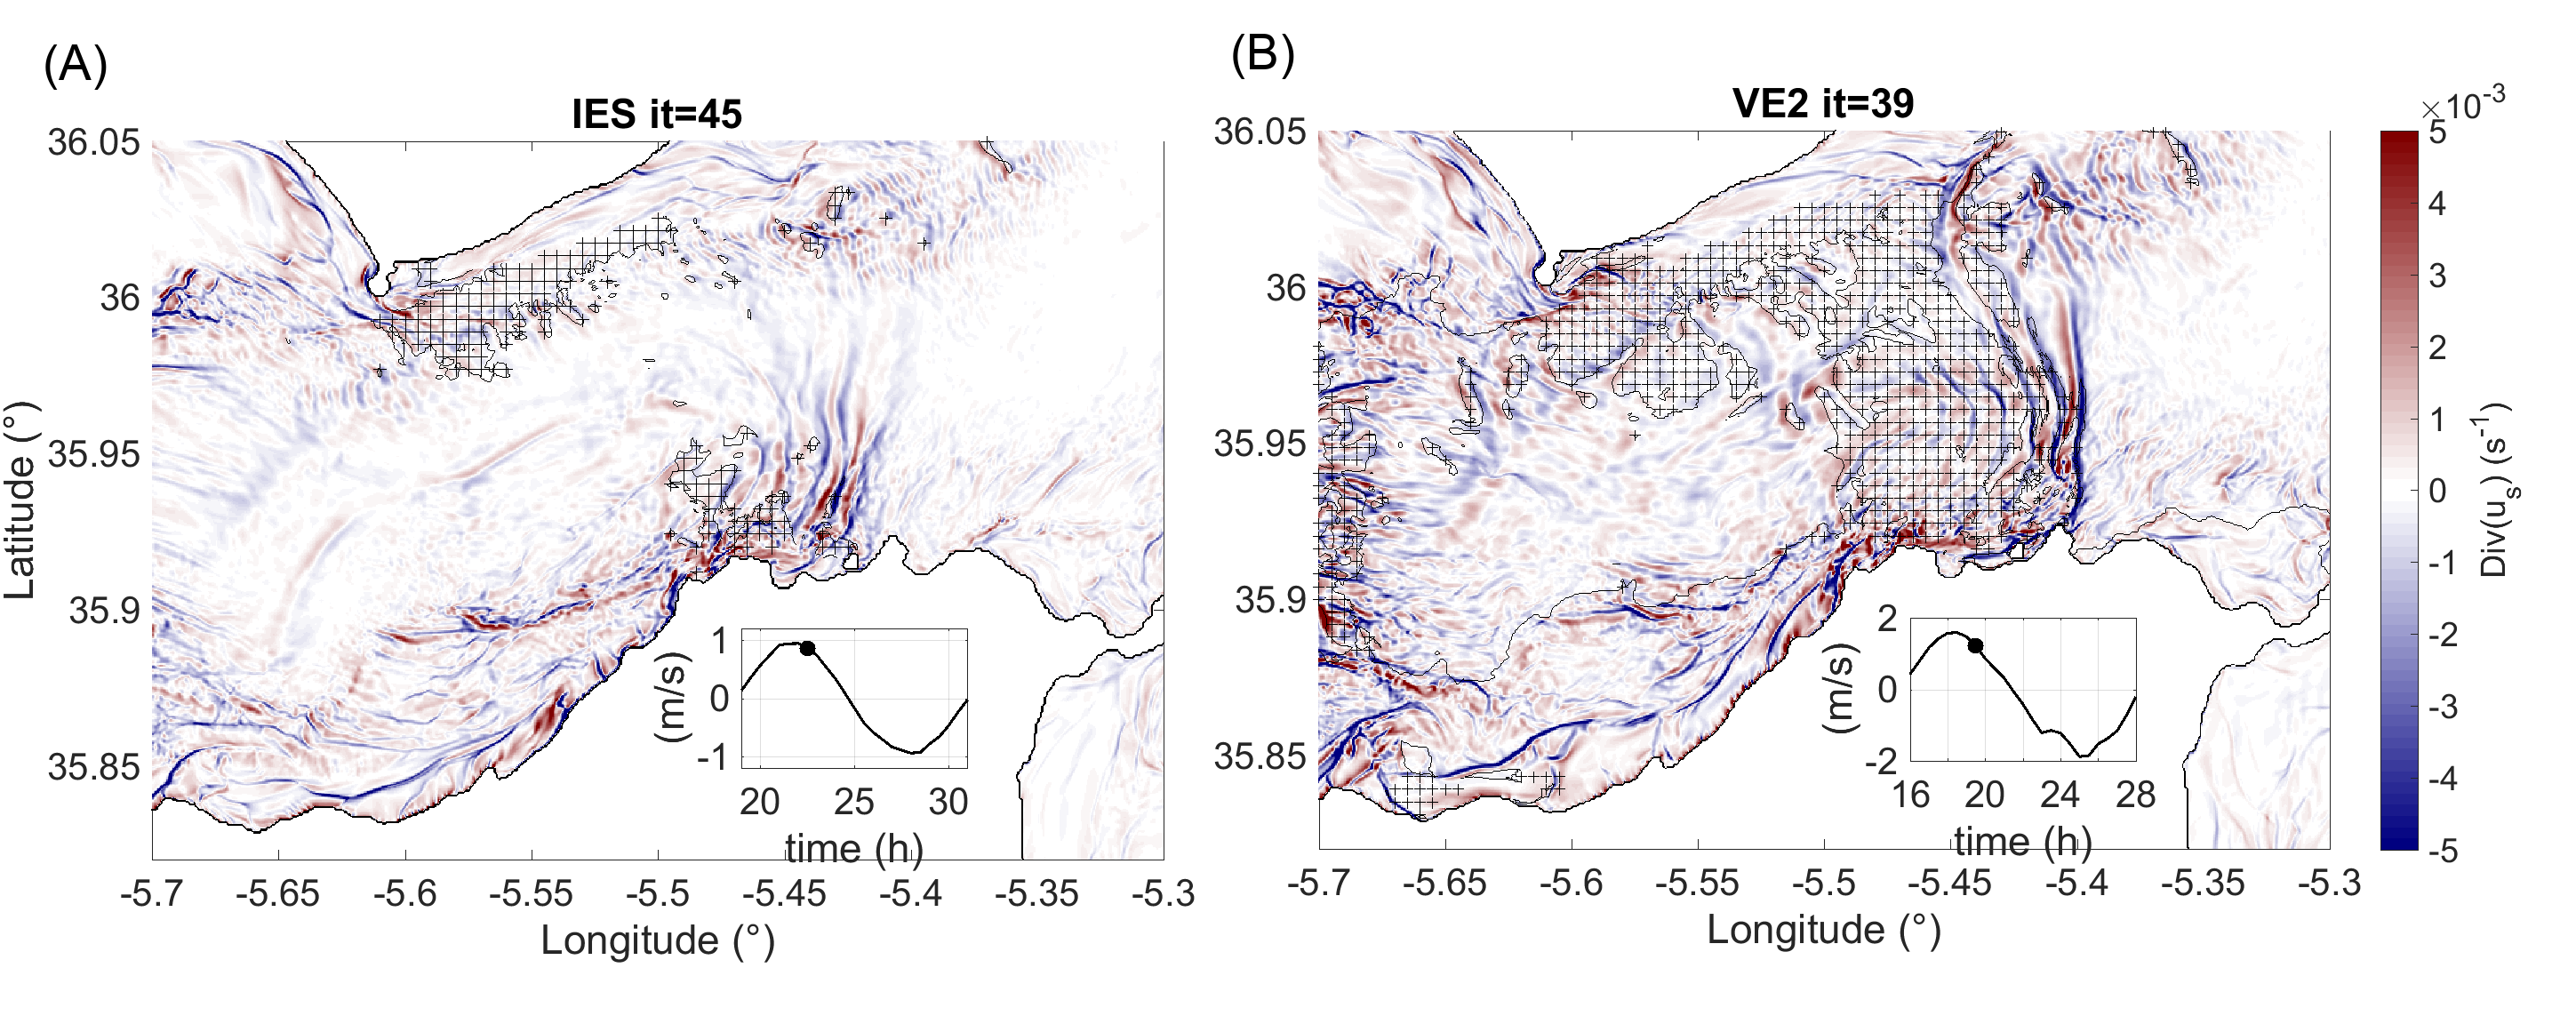
\includegraphics[width=\linewidth]{./GBR3D/FigWaveCont.png}
%\end{subfigure}
 \caption {Divergence of the surface current (color) and areas of supercritical Atlantic layer (black hatches) at t = 22.5 h in SimIT (a) and t = 19.5 h in SimST (b)}
 \label{FigISWGBR3D}
\end{figure}

\subsubsection{Propagation of Solitons (ISWs)}
\label{section_sim3D_ISW}

\begin{figure}[!h]
 \centering
 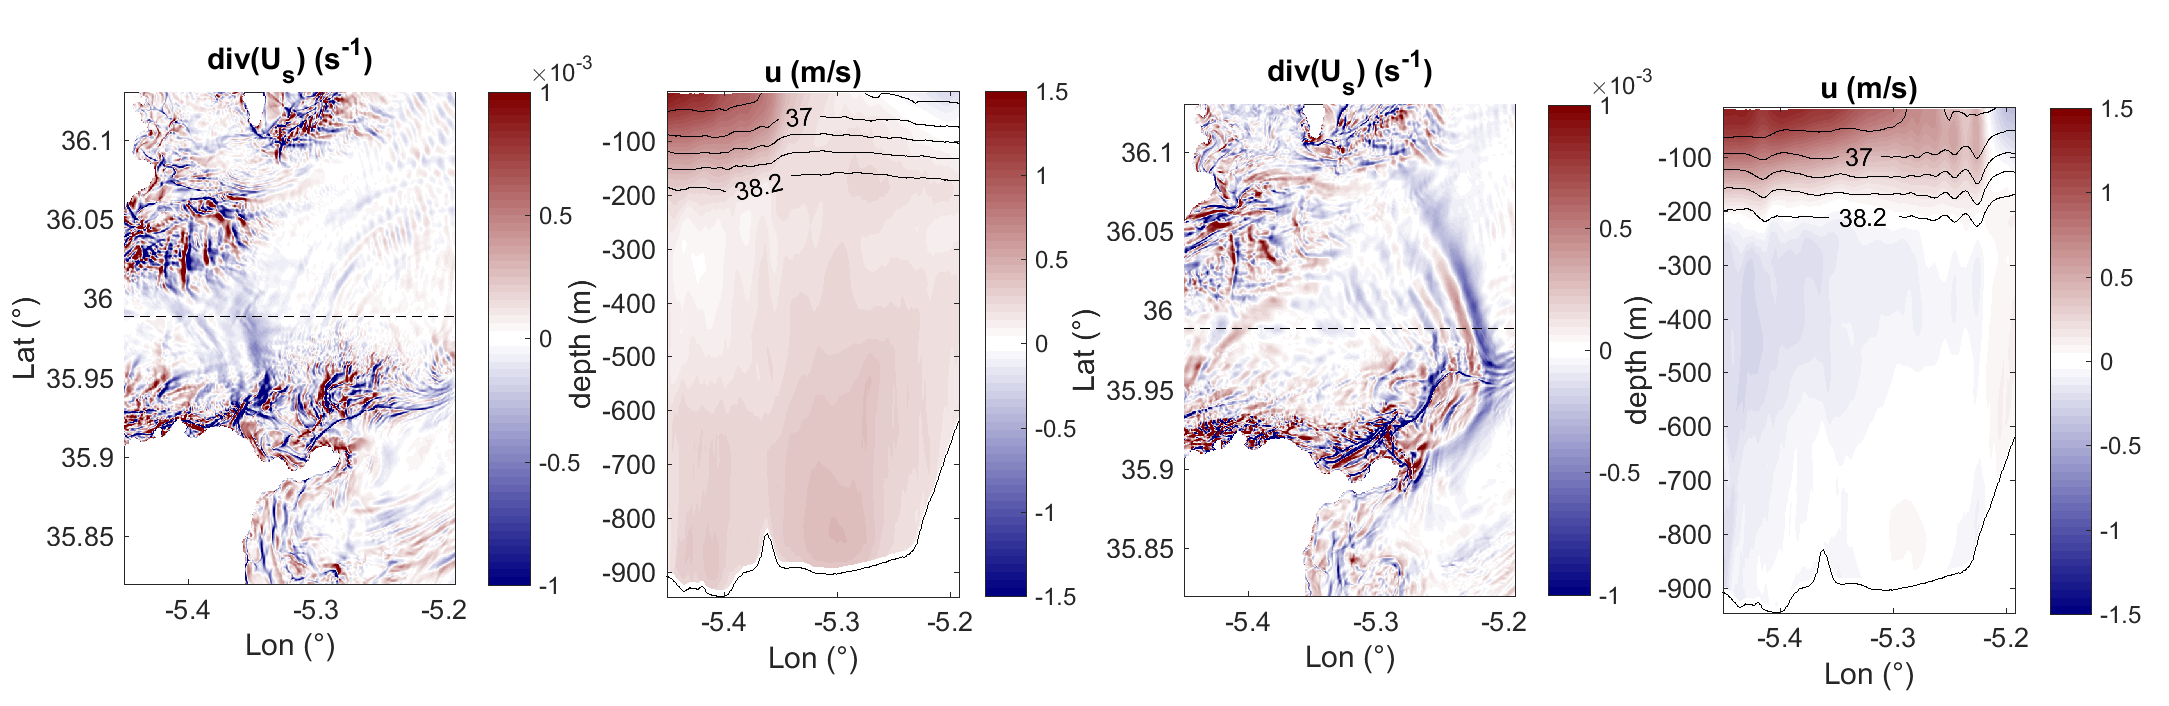
\includegraphics[width=1.\textwidth]{./GBR3D/coupesISW_ME2-2.png}
 \caption {Divergence of surface current (a, c) and vertical sections (b, d) of salinity (black isohalines) and zonal velocity $u$ (color) in SimNT at t = 20 h (a,b) and 22 h (c,d) of simulation.}
  \label{FigISWNT}
\end{figure}

\begin{figure}[!h]
 \centering
%\begin{subfigure}{\linewidth}
%\centering
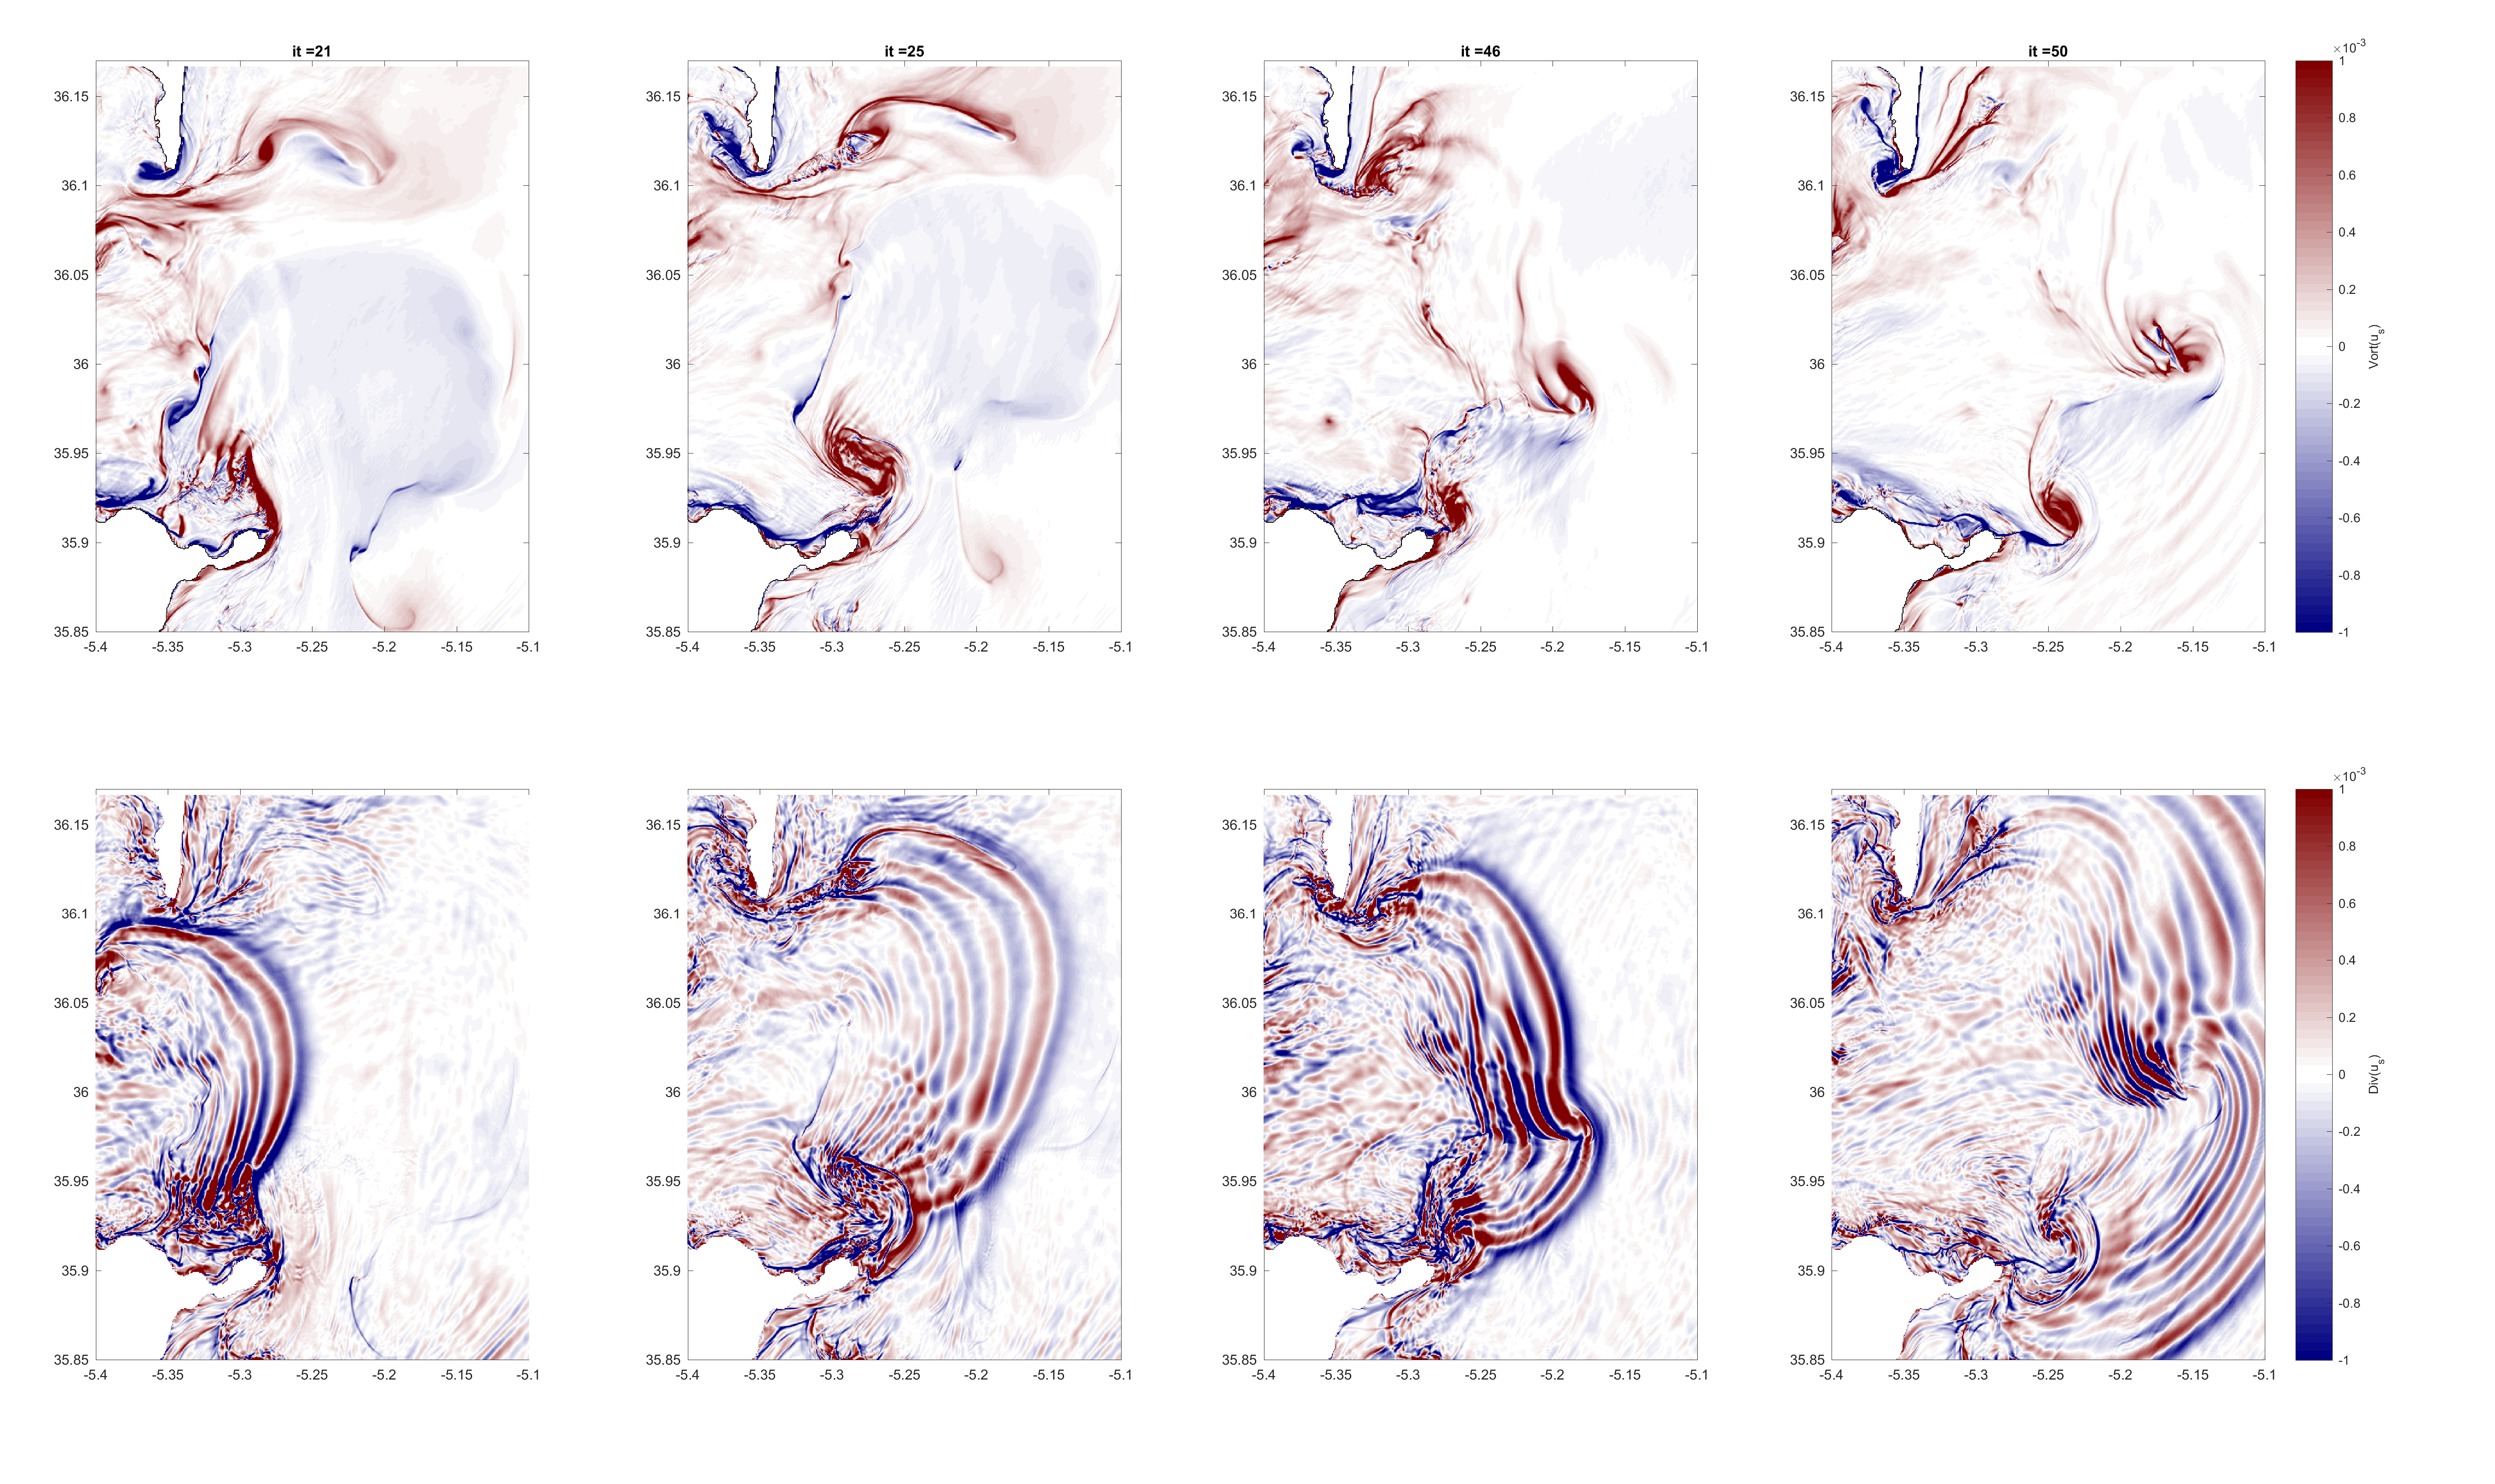
\includegraphics[width=\linewidth]{./GBR3D/FigTourbVE2.png}
%\end{subfigure}
 \caption {Divergence of surface current (upper row) at t = 10.5 h, 12.5 h, then 23 h and 25 h of simulation SimST, and z-axis vorticity of surface current (lower row) for the same time.}
 \label{FigeddGBR3D}
\end{figure}

Solitary waves are observed  \color{blue}after the relaxation of the hydraulic jump at CS (figure \noparref{FigISWGBR3D}). Figures (\noparref{FigISWNT}.a) and (\noparref{FigISWNT}.c) also depict the divergence of surface currents but at the eastern exit of the strait during the \color{black} inflow following a no-jump outflow. Figures (\noparref{FigISWNT}.b) and (\noparref{FigISWNT}.d) are vertical sections of the zonal current and salinity at the same date and time. A train of ISWs can be observed, this train ends up propagating in the Alboran sea. Meanwhile, the propagation of the baroclinic tide in figure \noparref{FigISWNT}.b creates a growing front \color{black} with isohalines steepening due to non-linear effects. As is the case for the ISWs generated at CS, the non-hydrostatic dispersion balances this effect and creates a train of ISWs. In SimNT this process occurs following every \textit{no-jump} outflows.

\color{blue}However, compared to the upper row of figure \ref{FigeddGBR3D} (also showing the divergence of surface currents during the tidal periods following the hydraulic jump at CS), the train of ISWs observed in the Alboran Sea after a \textit{no-jump} outflow is less extended and presents fewer solitons.  \color{black}

Figures (\noparref{FigeddGBR3D}.a-b) then (\noparref{FigeddGBR3D}.a-d) show two inflow periods separated by one tidal cycle in the SimST configuration. The lower row of \color{blue} figure \ref{FigeddGBR3D} exhibits the z-component of the surface vorticity \color{black} at the same time. In the first two figures of each row, a train of ISWs leaves the strait \color{blue} and enters into the Alboran sea. The number of solitons in the train increases during this period. \color{black} A filament of positive vorticity is formed by interaction with the southern coast in figure (\noparref{FigeddGBR3D}.e) and develops into a cyclonic eddy in (\noparref{FigeddGBR3D}.f).  \color{blue}In figure (\noparref{FigeddGBR3D}.c) one tidal cycle later, the eddy is located at 5.2 $^\text{o}$ W and 36$^\text{o}$ N and the new train of ISWs is refracted by this eddy: its southern part is indeed accelerated whereas its northern part is decelerated by the induced currents. At the same time, a vortical structure can be observed in the region of Ceuta. In figure (\noparref{FigeddGBR3D}.d) this structure has also evolved into \color{black} a cyclonic eddy that propagates in the Alboran sea. Meanwhile, the interaction between the solitary waves and the previous cyclonic eddy has resulted into an interference pattern in the wave packet. 

In the simulations, this process of generation of cyclonic eddies \color{blue} in the region of Ceuta \color{black} occurs each time a train of solitary waves exits the strait. The train of the next tidal cycle gets diffracted on this eddy, creating local \color{blue}modifications of the structure of the train. \color{black}

\subsubsection{Dynamical structures at Camarinal Sill, primary instabilities}
\label{sectionsim3D_res_insta}

\subparagraph{Neap-tide cycle.}
Along with the features of the flow already discussed previously, figures \ref{FigHCN}, \ref{FigHCS} and \ref{FigHCI} indicate patches of high standard deviation of parameter Q \color{blue} defined in (\S XXX). The extension of these patches is maximal during all outflow periods \color{black} and for the spring-tide inflow \color{green} (you mean "spring-tide flow"?), \color{black} although the values \color{green}(which values, standard deviations?) \color{black} for this latter case are not as large and the patch itself is not as extended. High values of the \color{blue} standard deviation \color{black} indicate the occurrence of large-amplitude oscillations of the values of parameter Q. \color{blue} Larger standard deviations can be found during the two outflow periods. Indeed during these periods, the hydraulic jump \color{black} is detected (\textit{w-jump} and \textit{s-jump}) west of CS at 5.79 $^\text{o}$ W and west of secondary bathymetric features in Tangier basin at 5.84 $^\text{o}$ W. There is also \color{blue} a smaller amplitude \color{black} signal at ES. It is of greater standard deviation for the spring tide outflow \color{green} (not sure to understand what you mean...). \color{black}

\color{blue}Figure (\noparref{FigTSCS}.a) superposes the standard deviation and \color{black} the singular vector of SVD performed on the 3D field of parameter Q computed during the outflow for the EOF explaining the largest part of the high-frequency variability, associated with propagation of vortices (the higher order EOFs (not shown) have low frequency variability and structure associated with the regional flow itself). \color{green}(la phrase est longue, longue... Tu peux la découper en phrases très courtes d'une part (j'ai essayé de commencer à le faire...) mais surtout commencer par un petit paragraphe d'explications/introductions sur ta SVD... Pourquoi, comment etc...) Je t'ai déjà mis une remarque sur ce point un peu plus haut. \color{black}

As expected, the contours of parameter Q  \color{blue}\sout{$=5e-5m^2s^{-2}$} $5x10^{-5}\ m^2s^{-2}$ plotted the \color{green}(which?) \color{blue} EOF are co-located with the values of large standard deviation, i.e. on the western slope of CS and on the western slope of secondary sills in Tangier Basin. \color{black} 

\color{blue}Figures (\noparref{FigTSCS}.b) to (\noparref{FigTSCS}.e) focuses on  \color{blue} a part \color{black} of the $\theta$-S diagram showing the signature of all the simulation grid-points at a given longitude zoomed in Mediterranean waters. Figure (\noparref{FigTSCS}.b) shows that at 5.76$^text{o}$ W, still over the crest of the sill, the spreading among Mediterranean waters remains similar to \color{black} the one found in figure \ref{Fig_Ini_WM3D} at the east entry of the strait. \color{blue}Figures (\noparref{FigTSCS}.c) and (\noparref{FigTSCS}.d) present the evolution of this $\theta$-S diagram along the path of what is becoming the Mediterranean outflow: \color{black} the water parcels are homogenizing and can be classified into three to four water masses.

These diagrams are \color{blue}more specifically \color{black} plotted for longitudes located in areas of large values of parameter Q, i.e. where mixing processes can be expected. However, clearly, Mediterranean water masses do not homogenize right after CS.  \color{green}Look into it with (tu n'as pas fini ta phrase???) \color{black}

\begin{figure}[!h]
% \centering
 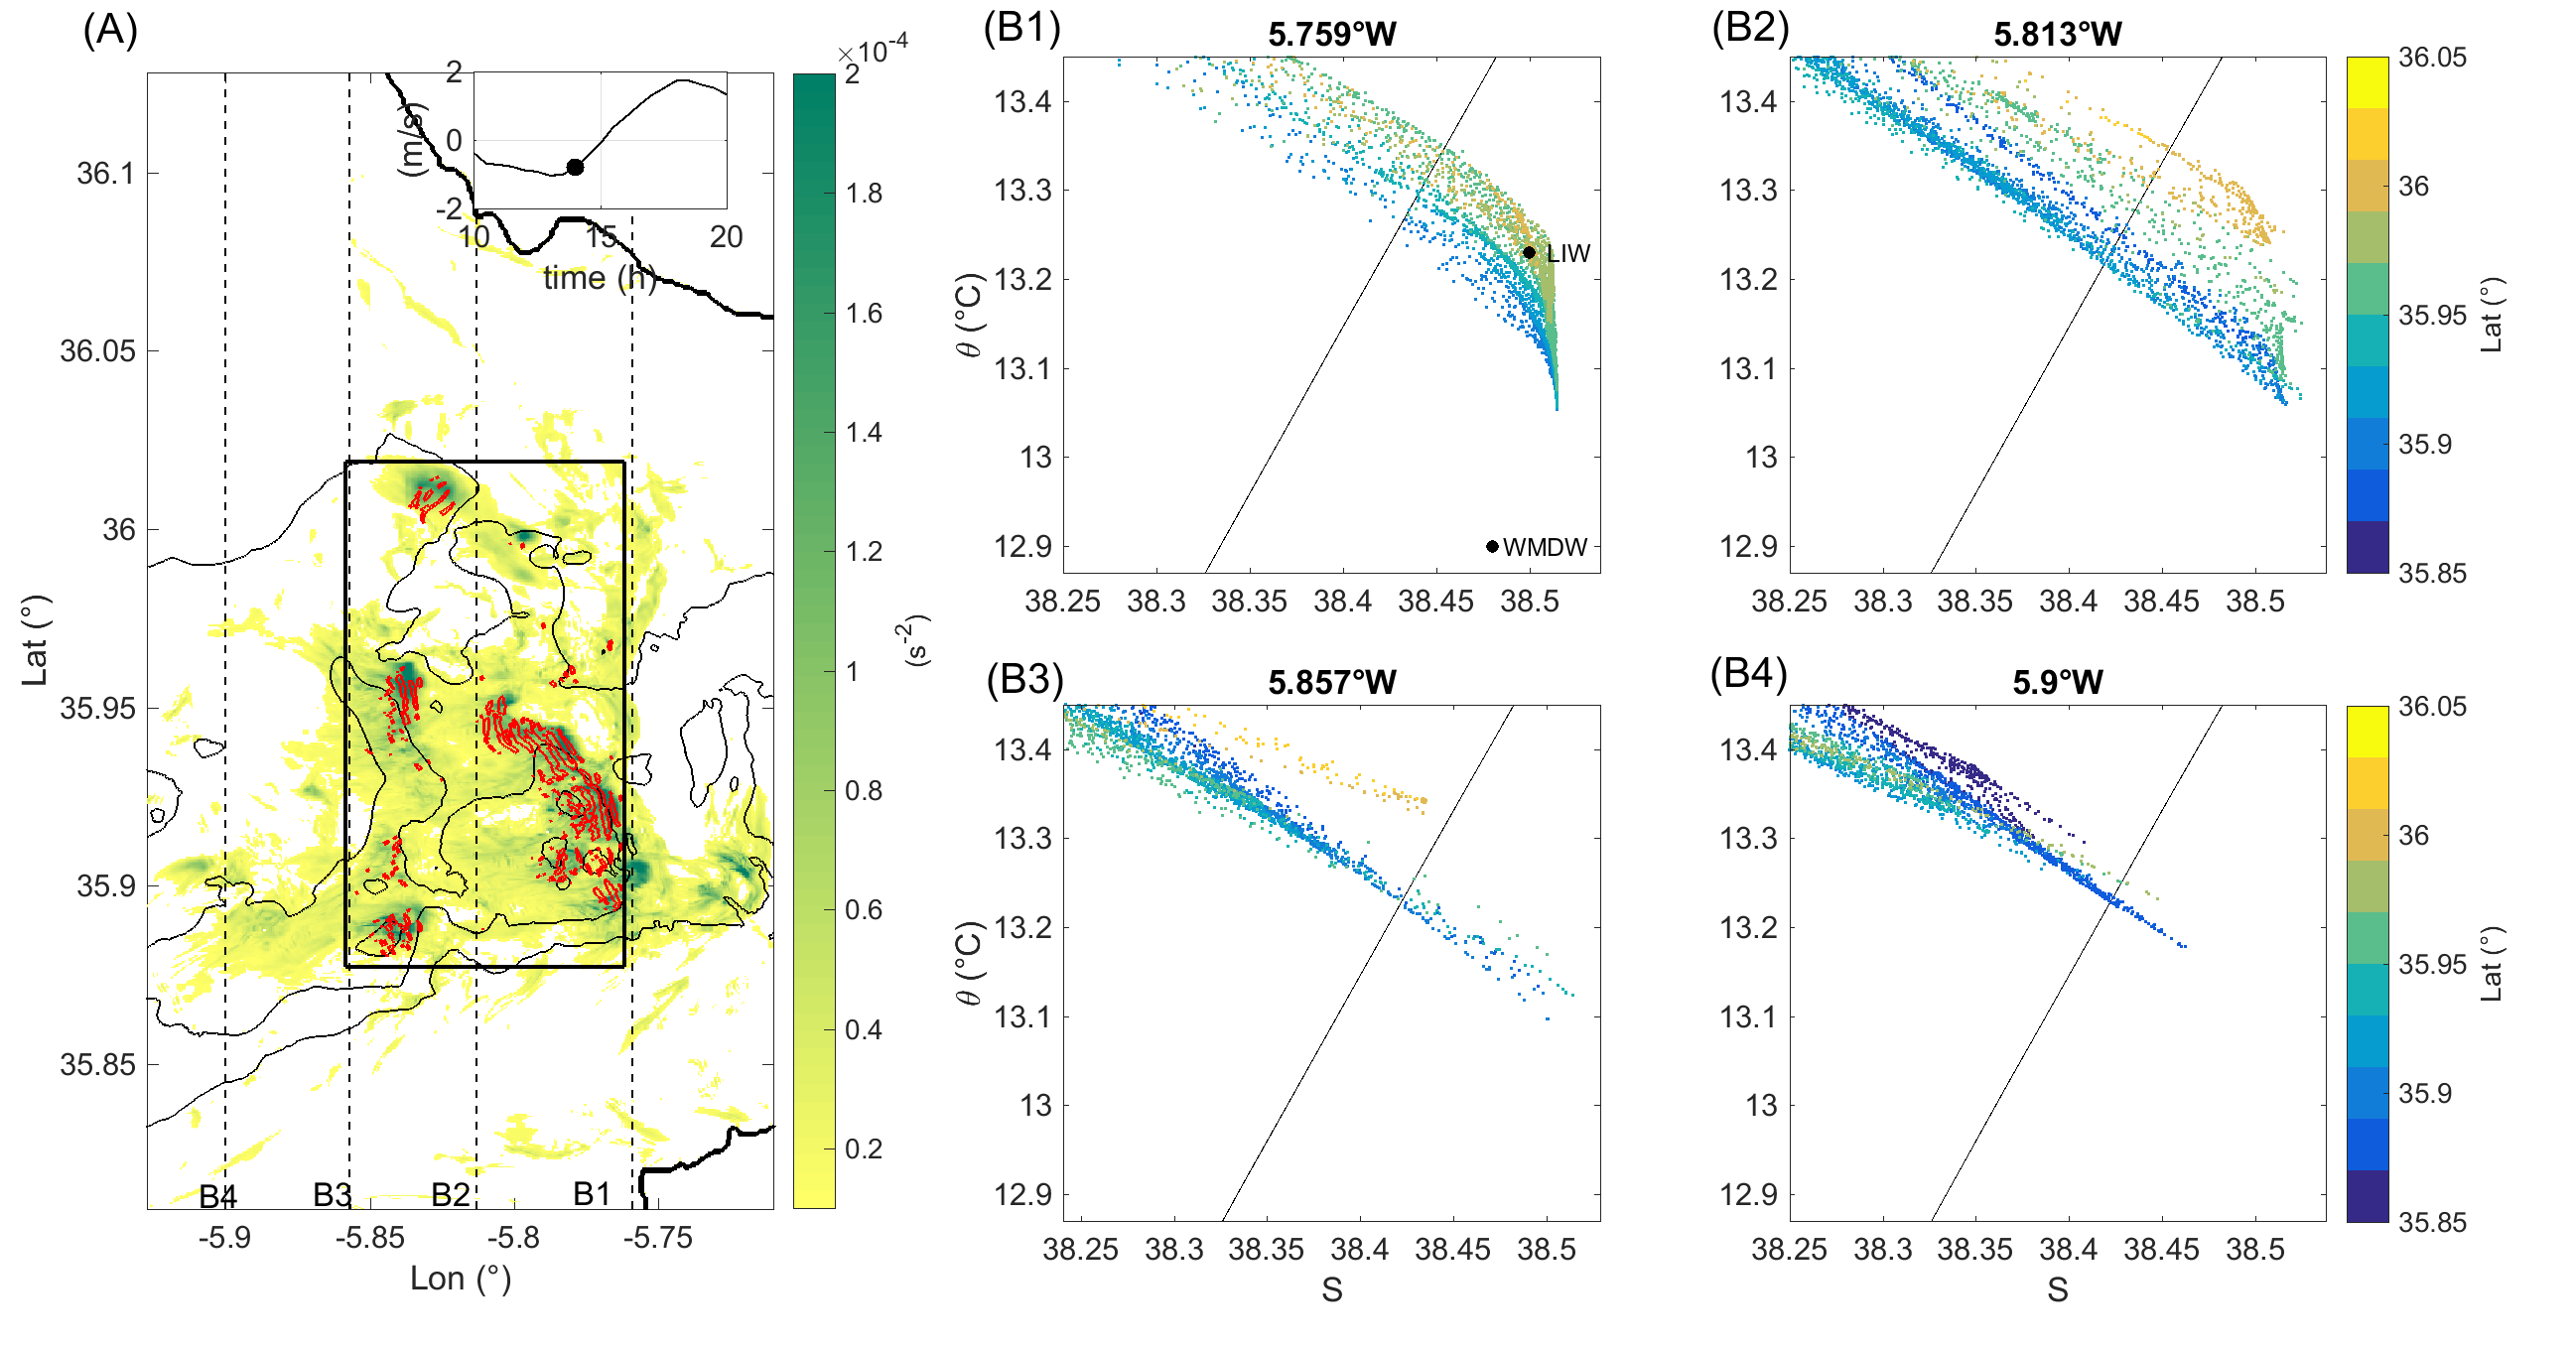
\includegraphics[width=\textwidth]{./GBR3D/TS_coupes_14H_VE2o.png}
 \caption {(a) Standard deviation of parameter Q over 30-mn-periods at $t\ =\ 14\ h$ in SimST (color) and trace \color{green}(what do you mean by trace? Isocontours?) of Q $\ =\ 5$\color{black} from the high-frequency EOF of SVD performed in the rectangular black box during the outflow period. Black dashed lines indicate the longitude at which $\theta-S$ diagrams are plotted. (b, c, d, e) $\theta-S$ diagrams, zoomed in the area of the Mediterranean water masses.  \color{green}(Mettre LETTRES, rajouter section plus au sud?) \color{black}}
 \label{FigTSCS}
\end{figure}

\color{blue}The singular vectors of SVD are now studied varying the strength of the outflows of barotropic tidal currents. \color{black} Figures (\noparref{FigEOFMIV}.a, b, c) present the EOF of parameter Q for the outflows of figures \ref{FigHCN}, \ref{FigHCS},and \ref{FigHCI}, along with vertical sections of salinity plotted \color{blue}at the same date and time \color{black} as figures (\noparref{FigEOFMIV}d,e,f). These sections are plotted along latitude 35.94$^\text{o}$ N. Figure (\noparref{FigEOFMIV}.g) and (\noparref{FigEOFMIV}.h) are histograms giving the height above the seafloor and the latitude of the grid points of the EOF for which Q is larger or equal to $5.10^{-5}\ m^2/s^2$. \color{green} (Attention: tu n'as pas mis d'unité par la suite pour Q... il faut les ajouter!) \color{black} On vertical sections, positive values of Q parameter are associated with specific billow structures of salinity that develop in the gravity current along the west slope of the CS. Those structures are generated for each outflow case, but the wider distributions of height above the sea floor and \sout{visualisation} in the vertical section \color{blue}indicate that \color{black} the billows \color{blue}\sout{have greater radius} are larger in \color{black} when and where an hydraulic jump is present, catching more interfacial and Atlantic waters into the Mediterranean outflow. At this longitude where the instabilities are still \color{blue}well-developed \color{black}, cores are not yet mixed in the simulation. A quick look at the $\theta$-S diagrams shows \color{blue} that the outflow is still heterogeneous.

The types \color{blue}of hydraulic jumps \color{black} also differ, while instabilities develop along the same areas in \textit{no-jump} and \textit{s-jump} case, in the w-jump case the hydraulic jump and the start of the gravity current are co-localised at all latitude as seen in the vertical section, which adds a possible area of generation between 35.92$^\text{o}$ N and 35.93$^\text{o}$ N, down slope of the shallowest point of the sill where the flow of Mediterranean waters is not as strong for \textit{s-jump} and \textit{no-jump} cases. \color{green} Difficile de suivre le raisonnement jusqu'au bout dans cette longue phrase. Peux-tu la reformuler un peu et la découper en trois ou quatre phrases très courtes ? (j'ai commencé pour aider...).\color{black}


\begin{figure}[!h]
% \centering
 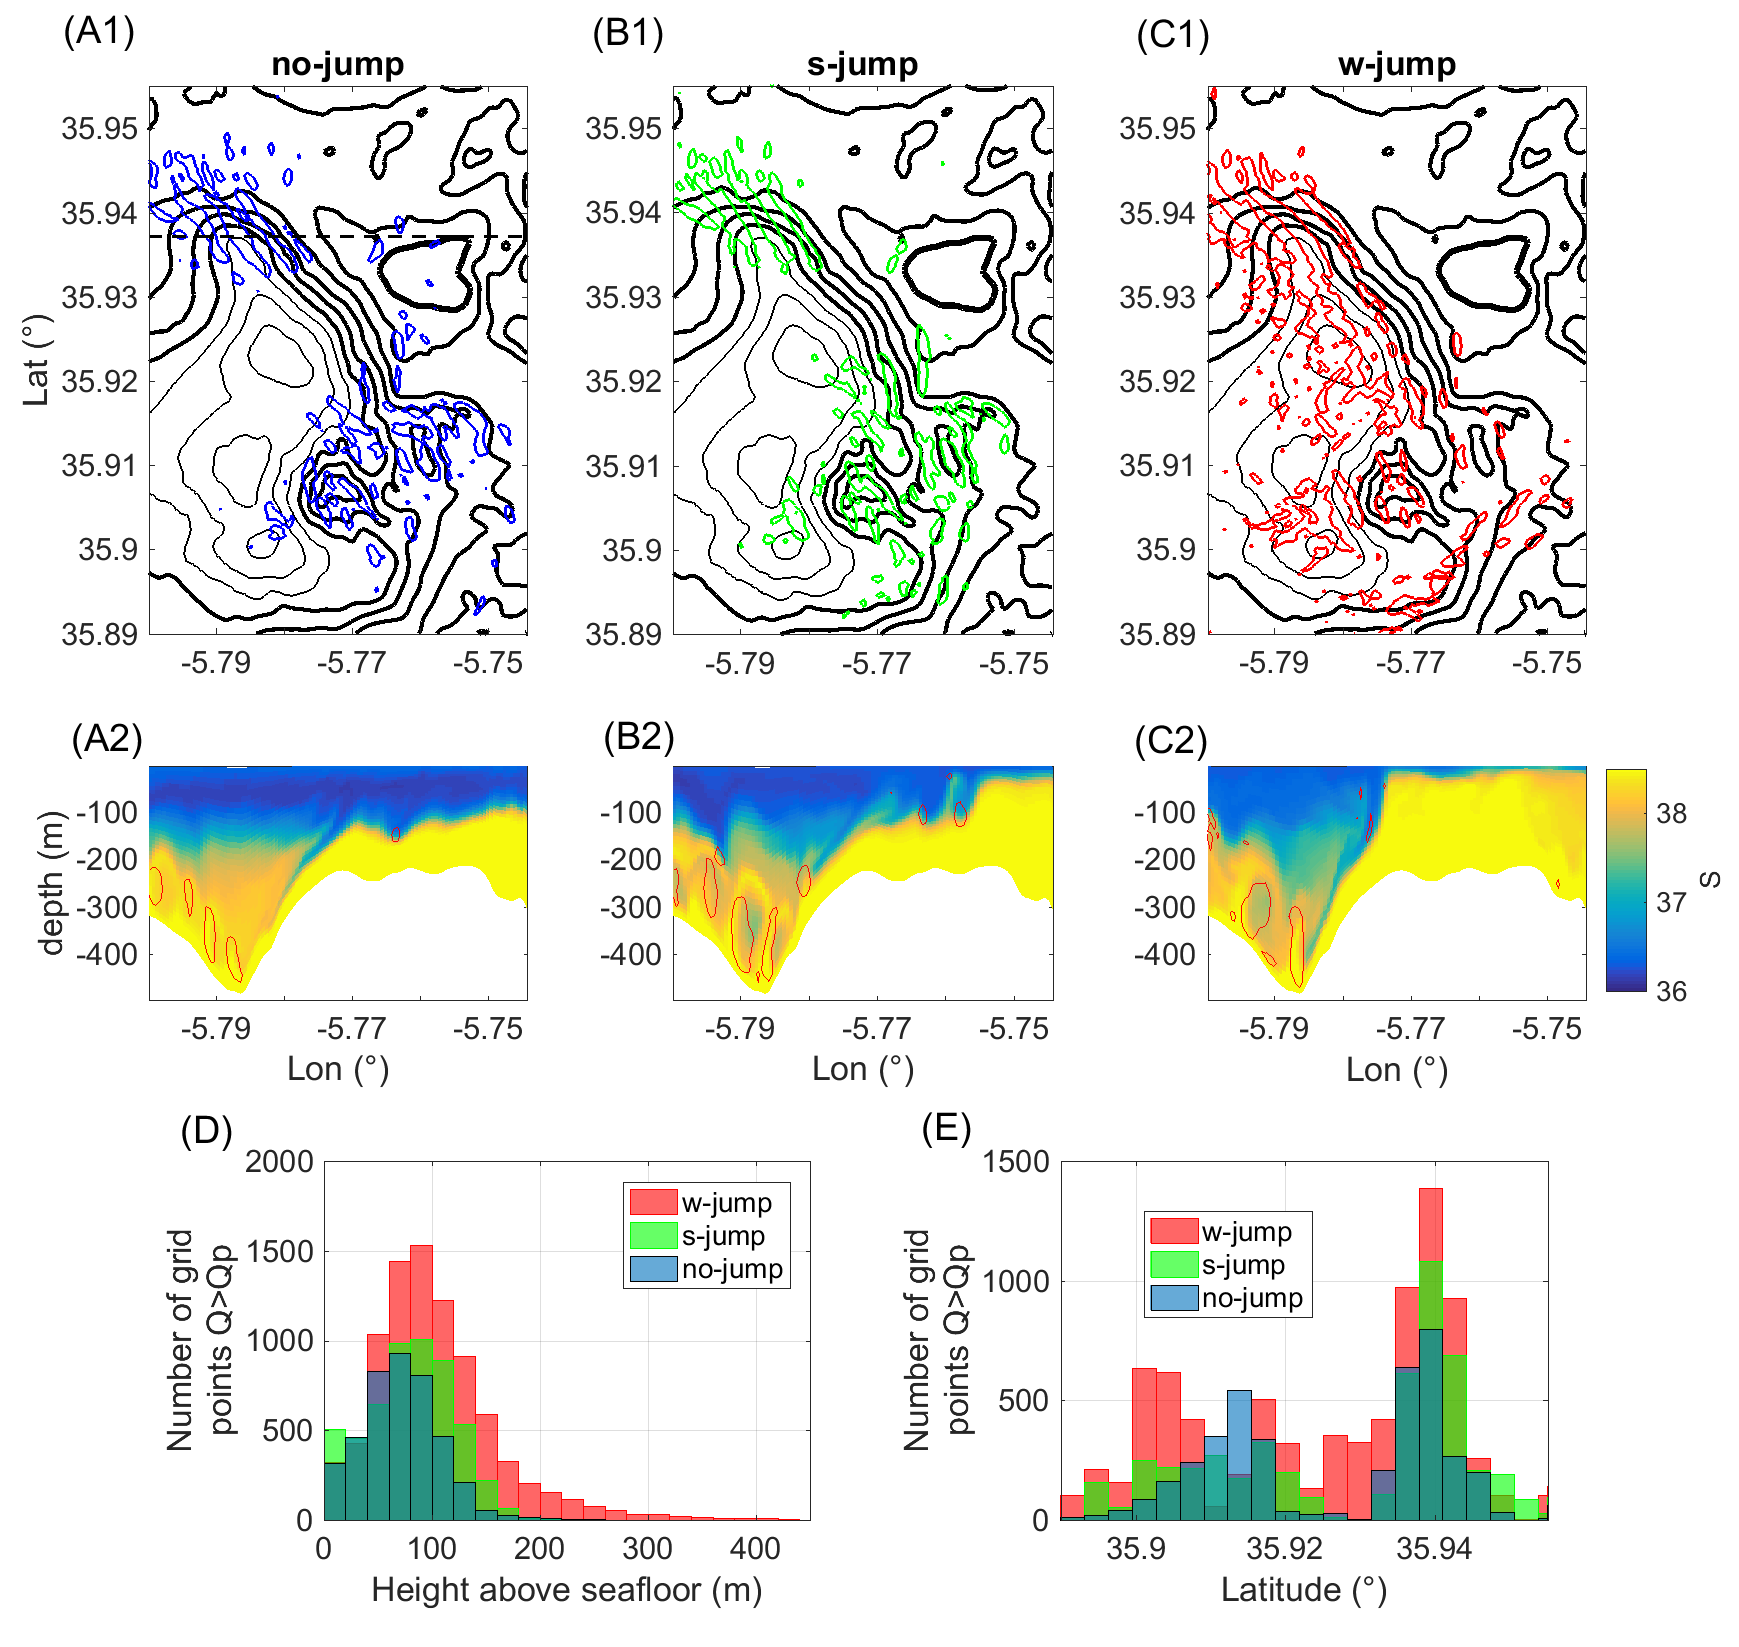
\includegraphics[width=\textwidth]{./GBR3D/EOF5_MIV_2D.png}
 \caption {(a, b, c) Contours of parameter Q$\ =\ 5.10^{-5}$ in first high-frequency EOF of SVD performed during outflow of figures (\noparref{FigHCN}.b),\ref{FigHCI} and (\noparref{FigHCS}.b) respectively. Isobathes in black: 200 m (thicker), 250 to 450 m (thick) and 500 to 600 m (thin). (d, e, f) Vertical sections of salinity (color) and contours of Q-parameter $\ =\ 5.10^{-5}$ at latitude $35.9372^\text{o}$ N at the same date and time as figures (\noparref{FigHCN}.b), \ref{FigHCI} and (\noparref{FigHCS}.b) respectively. (g) histogram of the height of the grid points of each EOF shown in a, b and c above the seafloor. (h) histogram of the latitude of the grid points of each EOF shown in a, b and c above the seafloor.}
 \label{FigEOFMIV}
\end{figure}

\subparagraph{Closure schemes.}

\color{blue}\sout{Now look at four other simulations, three use Smagorinsky turbulent scheme with different coefficients. One is using GLS K-$\epsilon$. .}
Four additional simulations are now presented to investigate and better understand the impact of the turbulent scheme: the first three are based on a different implementation of the Smakorinsky turbulent scheme and the latest uses the GLS K-$\epsilon$ scheme. \color{black}
\color{blue}In figure \noparref{Fig3Dsch}.a, c, e and g),\color{black} vertical sections of salinity during the first outflow \color{blue}after $t\ =\ 5\ h$ \color{black} of simulation which is in a \textit{no-jump} case, with indications of the values of the Richardson gradient number $Ri$ and Q parameter. $Ri$ is calculated from fields of density and velocity averaged over half and hour to filter out the propagating structures.

\color{blue}Figures (\noparref{Fig3Dsch}.b, d, f, and h) show the averaged salinity in Mediterranean (b, f) and Atlantic (d, h) layers, east (f,h) and west (b, d) \color{black} of CS. Note that averaged values are given and, as shown in figure \ref{FigTSCS} and in the vertical sections, the outflow Mediterranean layer is far from homogeneous at this longitude and at those longitudes. \color{black} \color{green}Je ne suis pas sûr d'avoir bien rendu ce que tu voulais dire ici? \color{black}

Looking at averaged layer salinities \color{green}(tu veux dire lorsque les salinités sont moyennées sur la couche, c'est cela?) \color{black} east of the sill in figures (\noparref{Fig3Dsch}.f and h), simulations SimIT-S001, SimIT-S01 and SimIT-Kep \color{blue} lead to the same salinities for the Mediterranean layer, whereas differences can be observed punctually in the Atlantic layer. The simulation presenting the largest differences is SimIT-S1: the Mediterranean layer is less saltier whereas the Atlantic layer is, in contrast, saltier. This is a direct consequence of the enhanced mixing coefficient which enhances mixing of these water masses in the pycnocline. \color{black}

\color{blue}However west of the sill in SimIT-S1, both the Atlantic and Mediterranean layers are saltier this time, especially between 2 and 8 hours following the initialization. This cannot obviously be explained by an increase of the dissipation.\color{black} After 5 hours of simulation, the vertical section shows that instabilities develop.  \color{blue}The area where $Ri$ is lower than $1/4$ begins at 5.77$^\text{o}$ W in all the simulations, indicating shear instabilities could develop from this point in the gravity current but instabilities can be found down slope of an intrusion of Atlantic waters at 5.783$^\text{o}$ W in simulation SimIT-S1. \color{black}
\sout{While the other simulations, the salinity entrained by the billows is from the altantic layer//contain less salty waters, ie the signal of atl surface water in the med outflow will be stronger in this simulation.} \color{green}(while ? do you mean unlike, whereas or in contrast..?) \color{black}
 \color{blue}In contrast, the billows are made of Atlantic water and, as a consequence, they are less salty. \color{black}
 
\color{blue}A larger proportion of Atlantic water is also incorporated in the bellows when $K-\epsilon$ turbulent scheme is implemented. \sout{Kepsilon}. Indeed, in this case the billows and more generally the instabilities are less-developped \sout{instabilitied} with smaller values of parameter Q  \sout{(closer to a gravity current only?) ???}, and a less-salty outflow. This signal persists \color{blue}$7\ h$ after the initialization when the flow reverses and no instabilities are generated any more. This process can also be observed but in a lesser extent in SimIT-S1 for which the effect of an increased diffusion in the pycnocline may counteract the injection of Mediterranean water. \color{black}

\sout{While} \color{blue}In simulations 1 and 2 (\color{green}1 \& 2?) \color{blue}, the width of the salty Mediterranean vein remains the same as it begins to go down slope of CS but instabilities arise earlier in the hydraulic jump and they bring more Atlantic water in the resulting billows. As these billows are advected down slope, more Atlantic water is integrated to the Mediterranean outflow when going through CS. \color{black} 


\begin{figure}[!h]
% \centering
 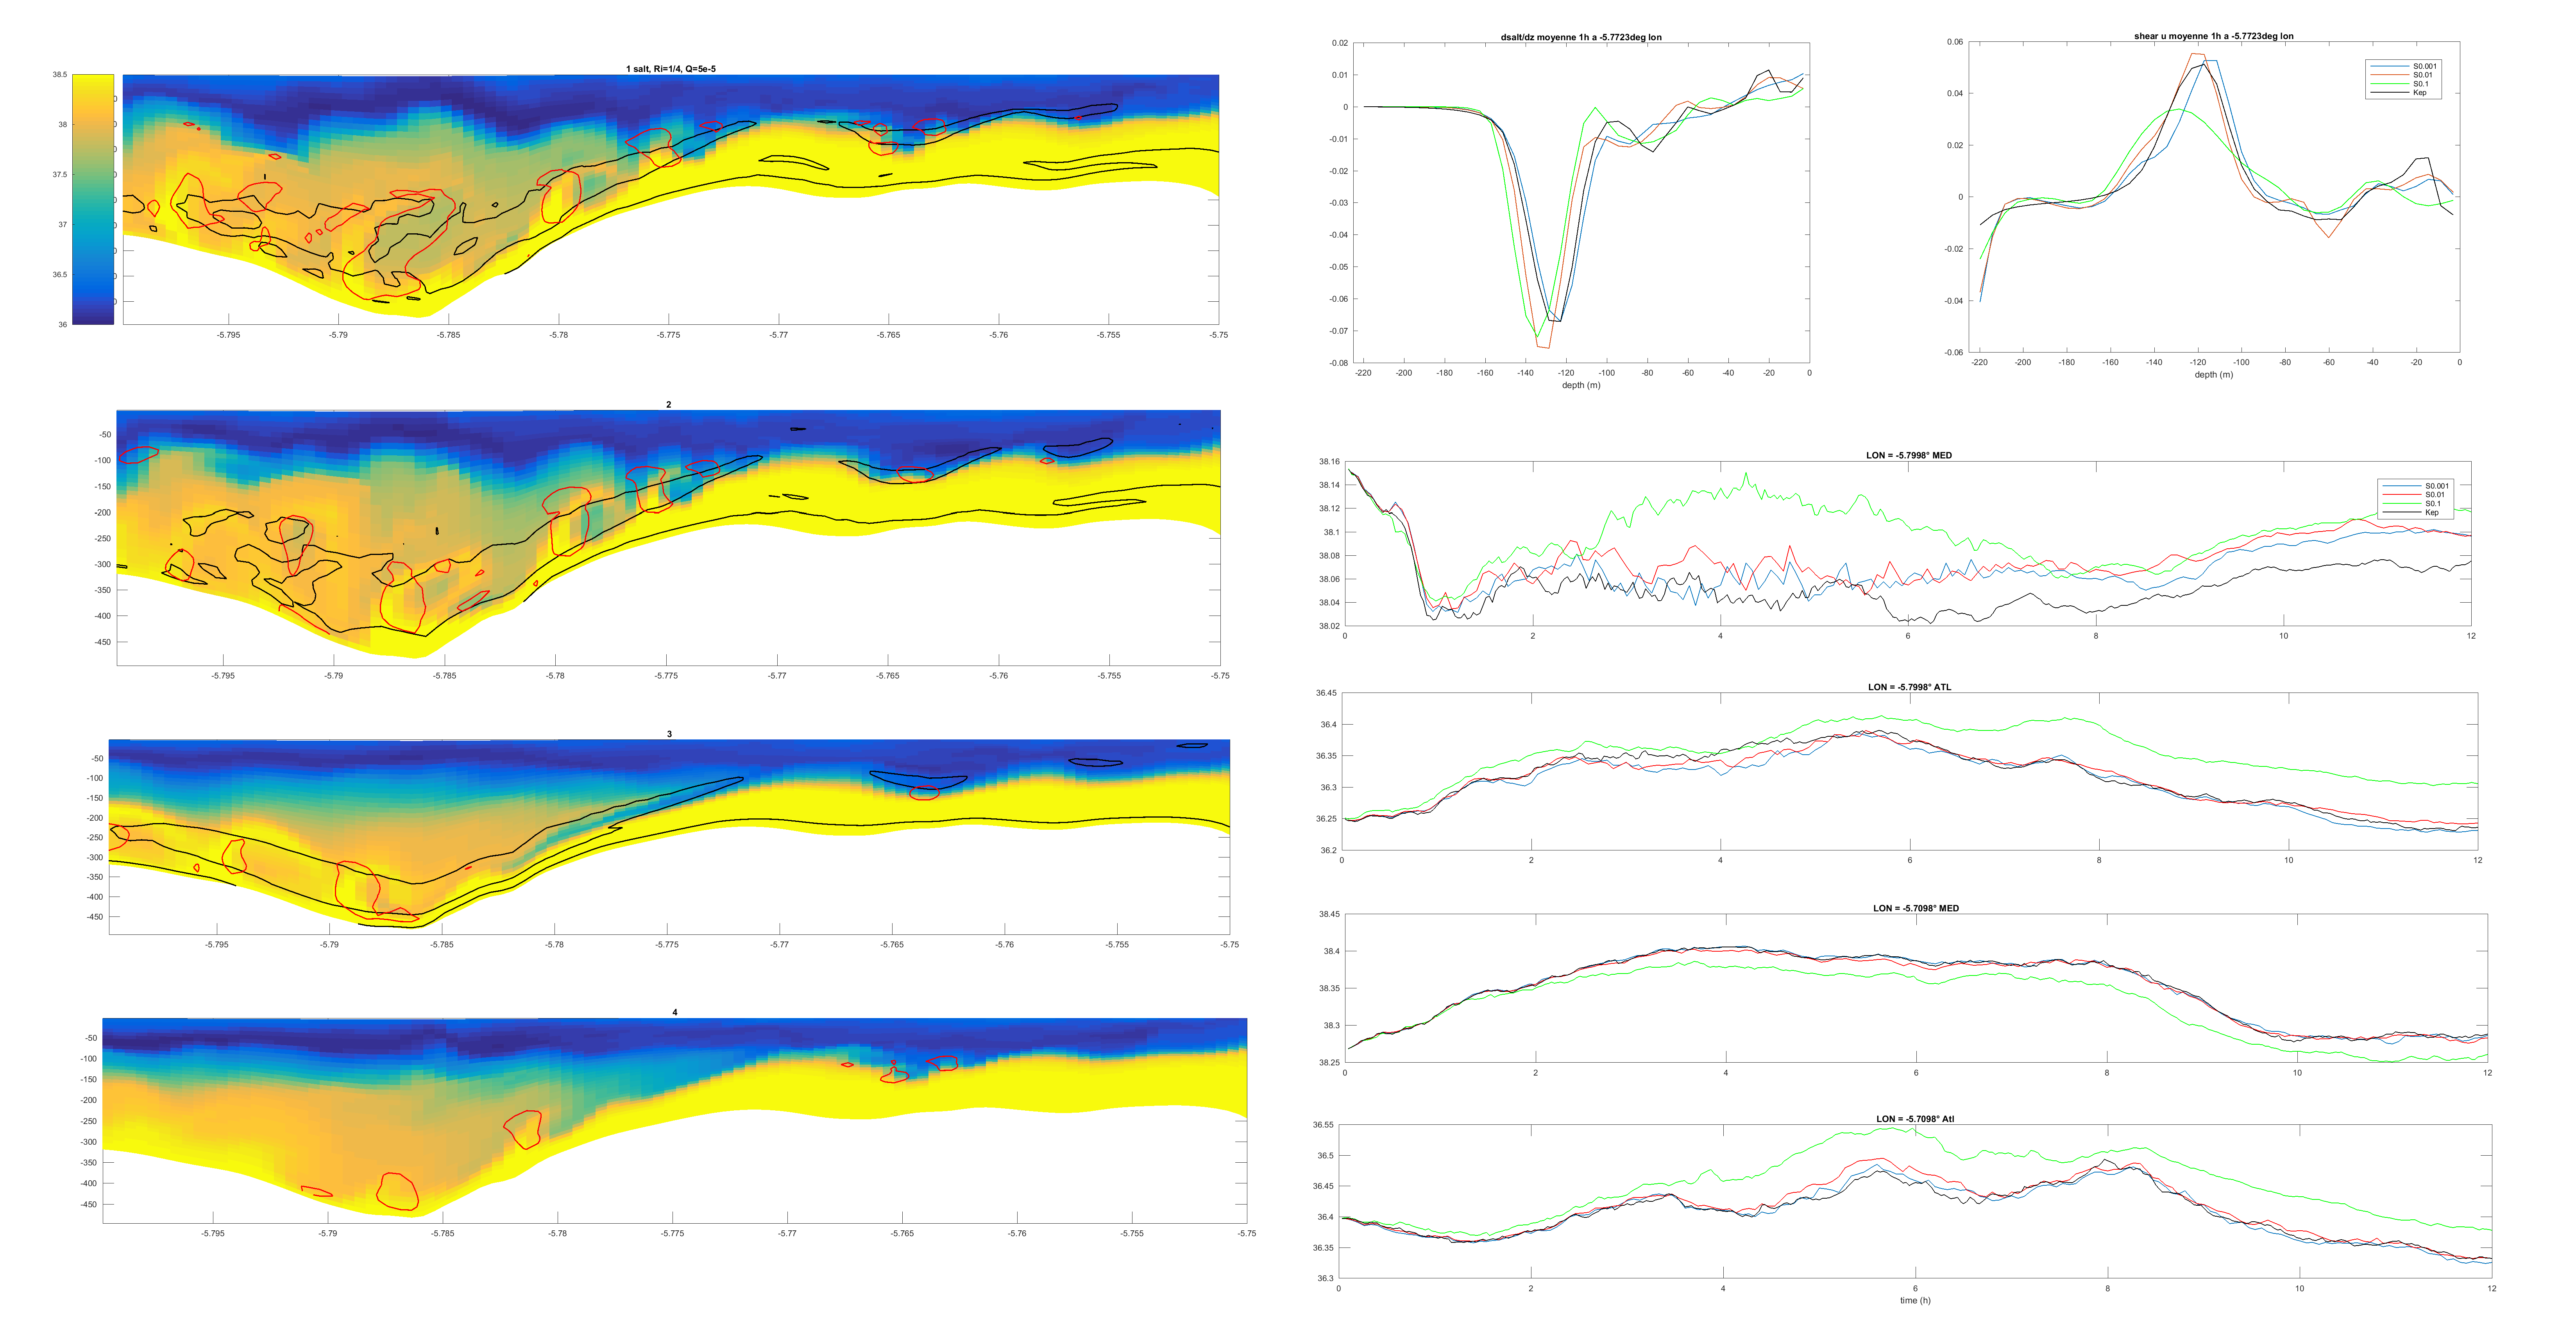
\includegraphics[width=\textwidth]{./GBR3D/Figsmago.png}
 \caption { \color{blue}vertical section of salinity (color), contours of $Q = 5.10^{-5}$ (red) and Richardson gradient number $=\ 1/4$ (black) at a latitude of $35.9372^o\ N$ in SimIT-S001, SimIT-S01, SimIT-S1 and SimIT-Kep IES, 4 h after the initialization.  \color{green}time  (1:S0.001  2:S0.01  3:S0.1 4:Kep)(Rajouter une évolution de ubar!!! sur s0.001) Je te laisse rédiger la fin. \color{black}}
 \label{Fig3Dsch}
\end{figure}

%----------------------------------------------------------------------
\subsection{Discussion \& conclusions}
%----------------------------------------------------------------------
\color{blue}\subparagraph{Fines scales in Gibraltar strait.}
\sout{Have looked into} The variability of the hydraulic control and of the other dynamical features during the neap-spring tidal cycle have been explored with high resolution, non-hydrostatic, free-surface simulations of the region of the Gibraltar strait. \sout{.See no permanent} No permanent supercritical flow has been identified in the various simulations and only intermittent events of such flows have been observed during the tidal cycle. The location and extension of the area of supercritical flow depend on the strength of the barotropic currents. \color{black}
\color{blue}During tidal outflows when both Atlantic and Mediterranean layers are critical, an hydraulic jump is generated and explicitly simulated. It is located \color{black} either over the shallowest part of the sill, or over its western slope.  \color{blue}This hydraulic jump evolves into a bore and then into a train of ISWs, as can be expected when the hydraulic control stops approaching high tide. The train of solitons finally leaves the strait into the Alboran sea. 
During tidal cycles with no critical flow over the sill and no hydraulic jump, the barotropic tidal signal induces a smaller (less extended) train of ISWs in the eastern part of the strait due to non-linearity. This train propagates into the Alboran Sea.  \color{green}J'ai eu du mal à comprendre, est-ce bien ce que tu voulais dire? \color{black}

 \color{blue}During \color{black} each simulated tidal cycle, a cyclonic eddy is formed along the coast of Ceuta (in the southern part of the eastern exit of the strait). This eddy is advected by the flow in the Alboran sea and interacts with the train of ISWs, \color{blue}inducing a local diffraction of the solitons. \color{black}


\color{blue}Several other dynamical features have been explicitly simulated such as the billows resulting from shear instabilities and developing\color{black} in the lee of CS. In simulations, these billows are associated to high positive values of parameter Q. This parameter is used as proxy for their detection and analysis. The billows are generated at the interface of \color{blue} Mediterranean and Atlantic waters and they are advected by the Mediterranean outflow. They are also present above secondary bathymetry accidents in Tangier basin and ES. They can be observed during outflows of any intensity, but their spreading changes with the intensity of tidal currents. They play an important role in the way the simulated Mediterranean and Atlantic waters mix, changing the hydrological features of the Mediterranean vein. The way this mixing occurs in simulations is sensitive to the dynamic of the instabilities and this dynamic is piloted by the turbulent dissipation scheme. \color{black}

\sout{Can see that} \color{blue}A conclusion is that the hydrological and dynamical properties of the Mediterranean waters entering in the northern Atlantic basin are greatly influenced by the configuration of the flow in the region of CS. Both the volume of these Mediterranean waters and their mixing with Atlantic waters can indeed vary during the neap-tide cycle. \color{black}
%the configuration of the flow at CS is the first passage of the Med waters, will affect the hydrological properties of the Mediterranean outflow, first by the volume of med waters that can flow west of the sill at each outflow, second by how much Atlantic waters are being mixed into it. 

%However, it is important to note that simulation only represents the beginning of the mixing by turbulent processes, in particular, no secondary evolution of KH instabilities.
\color{blue}In the present numerical configurations, only the largest primary instabilities and thus only the upper part of the turbulent direct cascade were explicitly simulated. The route to mixing consequently depends on the quality of the turbulence closure scheme used to end up mixing the water masses and this dependency has been evaluated by testing several schemes with well-known properties. 

%Moreover, the lack of atmospheric forcing probably means inaccuracies of features of the upper layer, especially circulation of the Atlantic layer in Tarifa Narrows where wind stress affects the upper layer. 
\color{blue}No atmospheric forcing were specified at the surface of the ocean in the configurations presented in this section. This means that the upper layer is not realistically represented in particular in the region of Tarifa Narrows where wind stress is particularly strong. This choice remains yet consistent with the desire to simplify (but not over simplify) the fine-structure dynamic in the complex region of the strait of Gibraltar. \color{black}

This choice could moreover explain why have the baroclinic tide degenerate into an internal bore and then into a train of ISWs during any inflows following a \textit{no-jump} outflow at CS, whereas observations \color{green}(cite tes sources) \color{black} indicate that during neap tides no solitary waves are generated. \color{green}(Ai-je bien compris ce que tu voulais dire ?). Other processes could be affected \color{blue} by the absence of atmospheric forcing \color{black} like the formation of eddies at the exit of the strait and their advection into \color{blue}the Alboran sea \color{black} that is probably influenced by the WAG.

\color{blue} \subparagraph{LES in Gibraltar strait.} To our knowledge (à vérifier en particulier à partir des dernières publications des romains!!!), the present study is the first 3D Large Eddy Simulation in the region of Gibraltar strait. We clearly do not claim that the primary instabilities have been explicitly simulated in the surface and bottom layers where the length-scales of these structures can be of the order of one meter or even less, i.e. still way too small to be simulated with a 50-m-resolution grid. However, what we claim is that Kelvin-Helmholtz instabilities have been explicitly simulated in the region of the interface between Mediterranean and Atlantic water masses. A resolution of a few tenths of meters both in the horizontal and vertical directions is enough in Gibraltar strait to do so in the middle of the water column. Compared to the kilometric horizontal-grid length-scales classically proposed, the much higher resolutions proposed here obviously lead to an increase of the computer coast to cover the region of the strait. This could be achieved thanks to the performances of the CROCO model inherited in part from ROMS time-splitting and numerical schemes \citep{shchepetkin_regional_2005} in which a non-hydrostatic, compressible kernel has been added \citep{auclair_non-hydrostatic_2018, hilt_numerical_2020}. This study is consequently a first step toward a downscaled, embedded, explicit simulation of the large turbulent structures when and where scale cascading leads to mixing in the water column.\\
The present work is thus a first LES exploration in \textit{Terra Incognita} \citep{scotti_large_2010, wyngaard_toward_2004}.\color{black}
\color{black}
